\resetdatestamp

\chapter{Turbulence impact on cloud droplet geometric collisions} \label{sec:ch2}

%\epigraph{The most beautiful thing we can experience is the mysterious. It is the source of all true art and science.}{\emph{Albert Einstein} (1879-1955)}
This chapter investigates and quantifies the turbulence effect on the droplet geometric collision rate. The goal of this chapter is to answer the following research questions: 1) What is the role of turbulence in droplet geometric collision (i.e., the collision that does not consider hydrodynamic droplet interactions)?  2) What is the relative importance of different scales of turbulent motion on droplet collisions? 3) Can we quantify the turbulent effects and find an accurate parameterization of the collision rate? At this stage, we are interested in the collision statistics that measure the relative velocity between droplets and the droplet clustering effect in various turbulent environments. The droplets are treated as ghost particles, i.e., droplets retain their original course of movement after collisions occur, so that the total droplet number concentration and droplet sizes do not evolve with time. It is demonstrated that turbulence exerts a positive impact on the droplet collisions. Meanwhile, a sensitivity test over a broad range of Reynolds number based on the computational domain size has been conducted to show that it has a negligible impact on the collision statistics. The implication is that the collision-related scales are very small and are well-resolved by the model. Past parameterizations of the turbulent collision kernel based on direct numerical simulation (DNS) included the Reynolds number as an important parameter and are of doubtful validity. Therefore, at the end of the chapter we propose a new parameterization that is indenpendent of the Reynolds number. 

This chapter consists of a paper published in the Journal of the Atmospheric Sciences: Sisi Chen, Peter Bartello, and M.K. Yau: Cloud droplet collisions in turbulent environment: collision statistics and parameterization, \url{https://doi.org/10.1175/JAS-D-15-0203.1}
\newpage

\section*{\centering Cloud droplet collisions in turbulent environment: collision statistics and parameterization}
\begin{center}
\author{Sisi Chen, Peter Bartello, M. K. Yau \\ \textit{Department of Atmospheric and Oceanic Sciences, McGill University, Montr\'{e}al, Qu\'{e}bec, Canada}\\ 
\and P.V. Vaillancourt \\ \textit{Meteorological Research Division, Environment and Climate Change Canada, Dorval, Qu\'{e}bec, Canada} \\}
\author{Kevin Zwijsen \\ \textit{Department of Atmospheric and Oceanic Sciences, McGill University, Montr\'{e}al, Qu\'{e}bec, Canada}}

\end{center}

\section*{\centering Abstract}
The purpose of this paper is to quantify the influence of turbulence in collision statistics by separately studying the impacts of computational domain sizes, eddy dissipation rates (EDRs), and droplet sizes and eventually to develop an accurate parameterization of collision kernels. Direct numerical simulations (DNS) were performed with a relatively wide range of EDRs and Taylor microscale Reynolds numbers $R_\lambda$ . EDR measures the turbulence intensity levels. DNS model studies have simulated homogeneous turbulence in a small domain in the cloud's adiabatic core. Clouds clearly have much larger scales than current DNS can simulate. For this reason, it is emphasized that $R_\lambda$ obtained from current DNS is fundamentally only a measure of the computational domain size for a given EDR and cannot completely describe the physical properties of cloud turbulence. Results show that the collision statistics are independent of the domain sizes and hence of the computational $R_\lambda$ for droplet sizes no bigger than 25 $\mu m$ as long as the droplet separation distance, which is on the order of the Kolmogorov scale in real clouds, is resolved. Instead, they are found to be highly correlated with EDRs and droplet sizes, and this correlation is used to formulate an improved parameterization scheme. The new scheme well represents the turbulent geometric collision kernel with a relative uncertainty of 14\%. A comparison between different parameterizations is made, and the formulas proposed here are shown to improve the fit to the collision statistics.

\section{Introduction} \label{sec:ch2_intro}
High-resolution simulations and in-situ measurements (such as observations by aircrafts) of cloud properties continue to advance our understanding of cloud and precipitation processes. However, difficulties persist in resolving certain puzzles in warm rain. Classical condensation theory stipulates that the growth rate of a cloud droplet radius is inversely proportional to the radius. As a result, a rain drop cannot be formed by condensation in a realistic time scale. Gravitational collision can speed up the growth process, but it is inefficient until a droplet attains a size of about 30 $\mu m$ \citep{Pruppacher1997}. Classical theory therefore is unable to account for the observed rapid onset of warm rain \citep{Szumowski1997, Knight2002}. Over the past two to three decades, a substantial amount of work has been conducted on studying the effect of turbulence on the generation of warm rain \citep[see the reviews by][]{Devenish2012,Grabowski2013}. Studies from laboratories \citep[for instance,][]{Fessler1994} and direct numerical simulations (DNS) \citep[for example,][]{Squires1991, Ayala2008a} have demonstrated that air turbulence can accelerate droplet collisional growth by increasing the relative velocity and enhancing coagulation effects. The large eddy simulation (LES) studies \citep[e.g., ][]{Seifert2010, Wyszogrodzki2013, Franklin2014, Grabowski2015} showed that turbulence can accelerate the onset of warm rain in shallow convective clouds as well as increase its intensity. However, most of the parameterizations of the turbulent collision kernels they used are a function of the Taylor-microscale Reynolds number, which is still under debate. Some studies used simplified turbulent collision efficiency (either assuming them equal to gravitational collision efficiency, or assuming them equal to unity in turbulent cases, or simply interpolating/extrapolating them based on only two turbulent cases.) In this paper, our focus is on the effects of turbulence on droplet growth by collision-coalescence and how sensitive is the collisional process to the Taylor-microscale Reynolds number.

It is known that there are three major effects of turbulence in enhancing the chance of droplet collision. The first one is the turbulent transport effect, which increases the droplet radial relative velocity (RRV) via the local shear and air acceleration. The second effect, termed the clustering effect, redistributes the cloud droplets such that they cluster in regions of low vorticity and high shear due to their inertia  \citep{Maxey1987, Wang1993, Reade2000, Vaillancourt2002}. \citet{Chen2006} proposed that clustering can also occur in regions of low Lagrangian acceleration.  The third effect is related to droplet-droplet aerodynamic interactions, which affect the collision efficiency. Because of the complexity of the problem and the lack of accurate and consistent representation of the disturbance flow in a turbulent background \citep{Rosa2011}, there are only a few DNS studies concerning this last effect \citep{Wang2005a, Ayala2007, Ayala2014}. Most of these treatments are still under development and remain computationally expensive.

To assess the effects of turbulence, there is a need to define the collision kernel, the relative velocity between droplets, and the degree of clustering. In a stagnant flow, the droplet collision rate is customarily described by the gravitational collision kernel: $K^g=\pi R^2|\mathbf{V_{t1}}-\mathbf{V_{t2}}|E(r_1, r_2)$, where R is the sum of the radii of droplets involved in collisions: $R= r_1+r_2$, $\mathbf{V_{t1}}$ and $\mathbf{V_{t2}}$ are the terminal velocities, and $E(r_1, r_2) $ is the collision efficiency. Since we are only concerned about the geometric collision kernel (collision without considering droplet-droplet interactions), $E(r_1, r_2) $ will not be pursued here. 

\citet{Saffman1956} introduced two expressions for the kinematic collision kernel by using cylindrical geometry and spherical geometry, respectively. The kernel denotes the surface of a droplet's swept-out volume within which collisions are expected to occur (see \citet{Wang1998b} for details). \citet{Sundaram1997} proposed a turbulent collision kernel as the product of \citet{Saffman1956}'s cylindrical form and the radial distribution function (RDF), g(R):
\begin{equation}
\Gamma ^{cyl}=\pi R^2 \langle|\mathbf{W}|\rangle g(R). \label{eqn:cyl}
\end{equation}
Here $\mathbf{W}$ is the relative velocity between two droplets when they collide. g(R) measures the clustering effect of turbulence, with values larger than unity if clustering is present. In stagnant air, $\mathbf{W}$ is just $\mathbf{V_{t1}}-\mathbf{V_{t2}}$, and g(R)=1 when droplets are uniformly distributed. \citet{Wang1998b} extended this turbulent collision kernel to a spherical form \eqref{eqn:sph} and demonstrated that this formulation is more appropriate for the turbulent case since the cylindrical form overpredicts the collision kernel by about $20\%$ or more.
\begin{equation}
\Gamma^{sph}=2\pi R^2 \langle|\mathbf{W_r}|\rangle g(R). \label{eqn:sph}
\end{equation}
Here $\mathbf{W_r}$ is the radial relative velocity (RRV) defined as $\mathbf{W_r} = \mathbf{W}\cdot \frac{\mathbf{R}}{|\mathbf{R}|}$, with $\mathbf{R}$ being the separation vector. 

It is widely accepted that the overall turbulent enhancement of collision statistics (i.e., the RRV, the RDF, and the collision kernel) depends on the turbulent eddy dissipation rate EDR ($\epsilon$) and the droplet Stokes number (St). The latter, defined as the ratio of the particle response time ($\tau_p$) to the Kolmogorov timescale ($\tau_k$), quantifies how fast a droplet reacts to the turbulent flow.

There are also a significant number of DNS studies demonstrating that the collision statistics are sensitive to the Taylor-microscale Reynolds number ($R_\lambda$). However, one should be very careful when interpreting their results as there are two types of $R_\lambda$ we use in the cloud community: one is real, the other is computational. By definition, $R_\lambda$ depends not only on the Taylor microscale, $\lambda$, but also on the turbulent fluctuating velocity at the largest scales. For the real $R_\lambda$, the largest scale is the overall size of the entire cloud; this $R_\lambda$, usually with an order of $\sim 10^4$ \citep{Pinsky2006collision}, represents the physical property of the cloud turbulence. Clearly, clouds have much larger scales than current DNS models can simulate. We, and previous authors, have merely simulated homogeneous turbulence in a small computational box, presumably located somewhere in the adiabatic core of the cloud. For this reason, the $R_\lambda$ obtained from these models refers only to the computational domain size, L; this computational $R_\lambda$, determined by the size of the domain, currently only attains values around $\sim 600$, or even less. \citet{Franklin2005} found collision statistics increased with both $R_\lambda$ and EDR from their DNS. Based on these simulations, \citet{Franklin2007} developed an empirical parameterization for the collision statistics that scales with $R_\lambda$. EDR terms were excluded from the parameterization by replacing them with $R_\lambda$ using an empirical power law fitted to their data (equation 12 in their original paper). Since this power law is only valid in their particular model configuration and cannot be applied to the general case, the replacement may not be justifiable. In their model configuration, $R_\lambda$ and EDR increased simultaneously and thus the separate effects given by EDR and $R_\lambda$ were unknown. Specifically, their L was fixed to 10 $cm$ for all simulations and kinetic energy was pumped into each simulation at a different rate to create different turbulent intensities. Accordingly, spatial resolution was modulated in such a way that the turbulent dissipation range (scales below the Kolmogorov length scale) would be well resolved.  However since EDR is negatively correlated to the Kolmogorove length scale, $\eta$, the scale separation between $\eta$ and L depends on the turbulent intensities. In this case, $R_\lambda$ is positively correlated with EDR such that the influence of the two cannot be separated. It follows that the cause of increments to the statistics was unclear. Therefore, a controlled study that can separate $\epsilon$ from $R_\lambda$ is called for.

\citet{Ayala2008a} found that the effect of $R_\lambda$ is secondary after reaching a certain value and the EDR effect is dominant. \citet{Rosa2012, Rosa2013} also found that collision statistics scaled with $R_\lambda$ but eventually reached an asymptotic value after $R_\lambda$ exceeded some threshold that depends on the size of the droplets involved in the collision. Collision statistics of small droplets ($r \leq 20 \mu$m) have smaller threshold values than large ones ($r \geq 30 \mu$m), since the latter have larger Stokes numbers and interact with a wider range of turbulent eddies.  However, \citet{Rosa2012} also commented that this $R_\lambda$-dependency was a result of "inadequate flow scale separation" in low-resolution simulations, because it only appeared at low $R_\lambda$. For this reason, caution should be exercised when interpreting the $R_\lambda$-dependency as the integral scale of the turbulence that determines the real Reynolds number of the cloud cannot be resolved by current DNS. In addition, previous DNS studies were either limited to a narrow range of domain sizes or to only a few dissipation rates (see table \ref{tab:DNS}). There is a need to extend these results to a wider range of parameters.

In the past few decades, there were several attempts to parameterize  the collision kernel but all show limitations \citep[see summary by][]{Ayala2008b}. They either excluded gravitational effects or clustering effects, or the results were only applicable to very large or small droplets or to a small range of $R_\lambda$. As discussed earlier, the $R_\lambda$ scaling in \citet{Franklin2007}'s empirical parameterization is inconclusive because the effect of EDR cannot be isolated. In addition, their parameterization is only applied to the cross-sized collision case as same-sized collisions (collisions between droplets with the same size) were not included in their model. \citet{Ayala2008b} derived analytical formulas for RRV and RDF, which also depend on $R_\lambda$. They extended the $R_\lambda$ range beyond the DNS limitation by taking into consideration the general representation of fluid velocity correlations in their formula. However, the integral length scale that determines the cloud-scale Reynolds number cannot be resolved by DNS, their parameterization might therefore be inaccurate. The parameterizations from \citet{Wang2000} and \citet{Zhou2001} also depend on $R_\lambda$ but were developed based on low-resolution runs that might not provide sufficient scale separation. $R_\lambda$ in \citet{Wang2000} ranges from 24 to 75, and \citet{Zhou2001} only studied the case of $R_\lambda$ = 45 and 58. \citet{Wang1998b} proposed a scaling law for the collision kernel and stated that it is independent of $R_\lambda$ when $R_\lambda$ is sufficiently large, as in the case of real clouds. 

This paper represents our continued exploration of cloud droplet collisions under turbulence begun by \citet{Franklin2005, Franklin2007}. Our purpose is 1) to better understand the influence of $R_\lambda$ on the collision statistics by separating its effect from that of the EDR, and to clarify the physical meaning of $R_\lambda$ in DNS; 2) to quantify the influence of turbulence intensity on cloud droplet collisions by simulating turbulent flow fields over a broad range of EDRs; 3) to seek a better parameterization for collision statistics with respect to different turbulent conditions. The paper is organized as follows. Section \ref{sec:ch2_model} describes the DNS model and the methods used; section \ref{sec:ch2_result} provides the results, showing that the collision statistics are independent of $R_\lambda$ while monotonically increasing with EDR. Based on these results we propose a new parameterization of the collision statistics in section \ref{sec:ch2_parameterization}; and section \ref{sec:ch2_conclusion} forms the summary and conclusion.


\begin{table}[ht]
\begin{center}
\def\arraystretch{1.5}
\caption{A summary of recent DNS studies on droplet collision statistics with turbulence.\strut} \label{tab:DNS}
\begin{tabular}{ccc}
\topline
 & $R_\lambda$ (number of grid points) & $\epsilon$ (cm$^2$ s$^{-3}$)\\
 \midline 
 \citet{Franklin2005} & $33-55$ ($80^3-240^3$) & $95 - 1535$\\
 \citet{Wang2008} & $43-72$ ($64^3 $ \& $128^3$) & $100$ \& $400$\\
 \citet{Ayala2008a} & $23-72$ ($32^3, 64^3,$ \& $128^3$) & $10, 100,$ \& $400$\\
 \citet{Rosa2013} & $28-303$ ($32^3-512^3$) & $400$\\
 \botline 
\end{tabular}
\end{center}
\end{table}


\section{Model and Methodology} \label{sec:ch2_model}

Our model mainly follows the framework of \citet{Franklin2005} and \citet{Vaillancourt2001}. A brief description is given below. Interested  readers may refer to the original papers for details.  Improvements and comparisons between our model configuration and that of \citet{Franklin2005} will be given in section \ref{sec:ch2_compares}.

\subsection{Flow, particles, and numerics}\label{sec:ch2_common}

The turbulent flow field was generated by solving the incompressible Navier-Stokes equations using a triply periodic pseudo-spectral technique (see Orszag 1969). The governing equations are 
\begin{equation} \label{eqn:NS1}
\frac{\partial \mathbf{U}}{\partial t}+(\mathbf{U}\cdot\nabla) \mathbf{U} = -\frac{1}{\rho_a}\nabla P+\nu \nabla^2\mathbf{U}+\mathbf{F}
\end{equation}

\begin{equation} \label{eqn:NS2}
\nabla\cdot\mathbf{U}=0, 
\end{equation}

where $\mathbf{U}$ is the turbulent flow velocity, $P$ is the pressure, $\nu = 1.6 \times 10^{-5} m^2 s^{-1}$, and $\mathbf{F}$ is an external forcing to maintain the turbulence. The turbulent flow was assumed statistically homogeneous and isotropic, as is the characteristic of the adiabatic cores of cumulus clouds \citep{Vaillancourt2000}. The adiabatic cores are regions free of entrainment and mixing with higher liquid water content than the rest of the cloud. Therefore, large droplets are expected to be found in these regions to initiate the collision and coalescence processes. To maintain statistical stationarity, the flow was forced in a low-wavenumber band following the approach of \citet{Sullivan1994} with $|\mathbf{k}|<k_f =1.5$, where $\mathbf{k}$ is the wave vector. This forcing was improved in order to maintain a more stable average EDR and details will be given in section \ref{sec:ch2_compares}.

As for the cloud droplets, radii in the range of 5 to 25 $\mu m$ were chosen as these sizes are critical to forming larger droplets to set the stage for effective collisional growth. For sizes smaller than 30 $\mu m$, Stokes drag law can be applied \citep{Pruppacher1997}. Since we assume no droplet-droplet aerodynamic interactions, the disturbance velocity field caused by the droplets was ignored. Thus the equation of droplet motion took on the simple form: 
\begin{equation} \label{eqn:dropmotion}
\frac{d\mathbf{V}(t)}{dt}=\frac{\tilde{\mathbf{U}}(\mathbf{X}(t),t)-\mathbf{V}(t)}{\tau_p}+\mathbf{g},
\end{equation}
where $\mathbf{V}(t)$ denotes the droplet velocity; $\tilde{\mathbf{U}}(\mathbf{X}(t),t)$ is the flow velocity at the droplet center position, which is the turbulent velocity $\mathbf{U}$; $\tau_p = (\frac{2\rho_w}{9\nu \rho_a}) r^2$, being the droplet response time and $r$ is the droplet radius; $\rho_a$ and $\rho_w$ are the density of air and droplet, respectively. $\big(\frac{2\rho_w}{9\nu \rho_a}\big) g=k$ was assumed constant with a value of $k=1.233 \times 10^8$ $m^{-1} s^{-1}$. Therefore, the droplet terminal velocities are calculated as $V_t = g \tau_p = k r^2$ for small droplets. 


To make our simulation close to reality, the initial droplet size distribution (DSD) of our poly-dispersive system was based on measurements made by \citet{Squires1958} for trade-wind cumulus clouds off the coast of Hawaii \citep[refer to fig. 5.9 in][]{Rogers1989}. In the simulations, droplets were randomly placed throughout the domain after the turbulence had reached statistical stationarity. At each droplet position the initial droplet velocity was given by the flow velocity obtained by linear interpolation \citep{Yeung1989}. To ensure that the initial conditions do not influence the results, droplets were given enough time (on the order of $100\tau_p$ for the largest droplet size)  to respond to the flow before compiling the collision statistics.


We used the cell index method \citep{Allen1987} to track droplet motions, following \citet{Franklin2005}. The droplets were treated as ghost particles, meaning they were allowed to pass through each other after the collision and continue their original course. This algorithm has been validated in detail in \citet{Franklin2005} and is shown to be consistent with the \citet{Saffman1956} formulation. Collisions were identified and counted by solving the quadratic equation (9) in \citet{Franklin2005}.

Three statistics were examined to measure the turbulent effects on droplet collisions: the collision kernel, the RDF, and the RRV.
The definition of RRV was given in section \ref{sec:ch2_intro}, and the RDF is defined as:
\begin{equation}
g(R)=\frac{N_p\Omega}{V_sN_tN_1N_2},
\end{equation}
where $\Omega$ is the domain size; $N_1$ and $N_2$ are the number of droplets from the two different size groups in the domain (for same-sized collision, $N_1N_2$ becomes $\frac{N^2}{2}$); $N_t$ is the number of time steps; $N_p$ is the number of pairs at contact found in the shell volume $V_s=\frac{4\pi}{3}[(R+R/100)^3-(R-R/100)^3]$ within $N_t$. The shell volume had an outer radius slightly larger than R to allow enough sampling of droplet pairs at finite $N_t$. It is safe to do so because very little dependence of the RDF on the shell size is found as long as the outer radius is smaller than 1.1R \citep{Wang1998b}. 

In addition to its kinematic equation shown in (\ref{eqn:sph}), the collision kernel can also be computed by dynamically counting the number of collisions that take place during the simulation:
\begin{equation}
\Gamma^{dyn}=\frac{N_c\Omega}{N_1N_2N_t\Delta t},
\end{equation}
where $N_c$ is the number of collisions and $\Delta t$ is the time step.

\subsection{Model improvements and validation} \label{sec:ch2_compares}

\subsubsection{Expansion of the domain size: MPI technique and validation} \label{sec:ch2_mpi}

To run simulations with larger box sizes, we used the Message Passing Interface (MPI) for parallelization instead of the OpenMP interface in the code of \citet{Franklin2005}. The drawback of OpenMP is that it requires shared-memory machines with a small number of processors. On the other hand, the MPI technique can be used in both shared and distributed memory architectures and therefore allows a much larger number of processors. We used a one-dimensional decomposition technique to divide the computational domain equally in the $y$-direction into vertical slabs, such that each processor works on one slab. With this technique we performed simulations with $R_\lambda$ up to 589. Local dissipation rates of shallow cumulus clouds in the incipient or decaying region are usually moderate with values around 10-100 $cm^2s^{-3}$ \citep{Seifert2010}. Numerical studies show that the highest local dissipation rates can sometimes reach a few thousand at some regions of clouds \citep{Franklin2014, Benmoshe2014}. Therefore, the EDR used here spanned the range from 50 to 1500 cm$^2$ s$^{-3}$.

To validate our MPI-based code, two tests have been performed with the following configuration. We fixed the box size to $L=0.1$ m in the $x$, $y$, and $z$ directions. $25,000$ droplets with a radius of 10 $\mu m$ and the same number of droplets of 20 $\mu m$ were placed randomly into the domain. The liquid water content was approximately 1 $gm^{-3}$, which is close to the typical value found in adiabatic cloud cores.

The first test was to validate the droplet tracking and collision detection scheme. To simplify the case turbulence was turned off so that droplet motion was only driven by gravity along the $z$-axis. The number of grid points was set to $240^3$. Since the spatial distribution of droplets in the $xy$-plane does not change in time without turbulence, the initial condition for a single realization strongly affects our statistics. To avoid this problem 20 realizations with different random initial droplet positions were used and collision statistics were calculated from the ensemble average.  We obtained an average RDF of $g(R)^{avg}=1.0276$ and an average collision kernel of $\Gamma^{avg}=1.0320\times 10^{-10}$ $m^3 s^{-1}$. These values are  close to the respective theoretical values ($g(R)=1$ for a uniformly distributed case, and $\Gamma^{sph} = 1.0459\times 10^{-10}$ $m^3 s^{-1}$ according to formula (\ref{eqn:sph})), with only $\pm$ 3\% of difference.

Restoring the turbulence, the second test was to find a justifiable value of $k_{max}\eta$, where $k_{max}$ is the maximum resolvable wave-number. In order to resolve the smallest scales of turbulence, while at the same time avoiding unnecessary computations on non-contributing scales far below the Kolmogorov length scale, we should minimize $k_{max}\eta$, while keeping it larger than unity. Fifteen different simulations were performed with different numbers of grid points varying from $16^3$ up to $240^3$ and with a fixed EDR of 1000 cm$^2$ s$^{-3}$. In so doing the turbulent flow parameters (such as the root-mean-square velocity $u\prime$, $R_\lambda$, $\eta$, etc.) remained identical, and grid size ($\Delta x$) became the only factor influencing our collision statistics. With the grid size changing $k_{max}\eta$, spanned a range of $0.2-3.4$, covering most values used by other researchers \citep{Ayala2008a, Franklin2005, Wang1993, Yeung1989}. Figure \ref{fig:kmaxeta1} illustrates the dependence of the collision kernel and RDF on $k_{max}\eta$. All values were normalized by their respective averages over the data points with $k_{max}\eta>1$. As shown in the figure, the collision statistics varied within $\pm 2\%$ from the mean after $k_{max}\eta \approx 1.0$. To be on the safe side we settled on a value of $1.3$ in all our subsequent simulations. Note that $k_{max}$ is determined solely by $\Delta x$ since $k_{max}=(2/3)\frac{2\pi}{2 \Delta x}$ in our dealiased pseudo-spectral code, and $\eta$ solely by the EDR since $\eta = (\frac{\nu^3}{\epsilon})^{1/4}$. It follows that a one-to-one correspondence can be established between $\Delta x$ and $\epsilon$ once we fix the value of $k_{max}\eta$. 

\begin{figure}[ht]
\centering
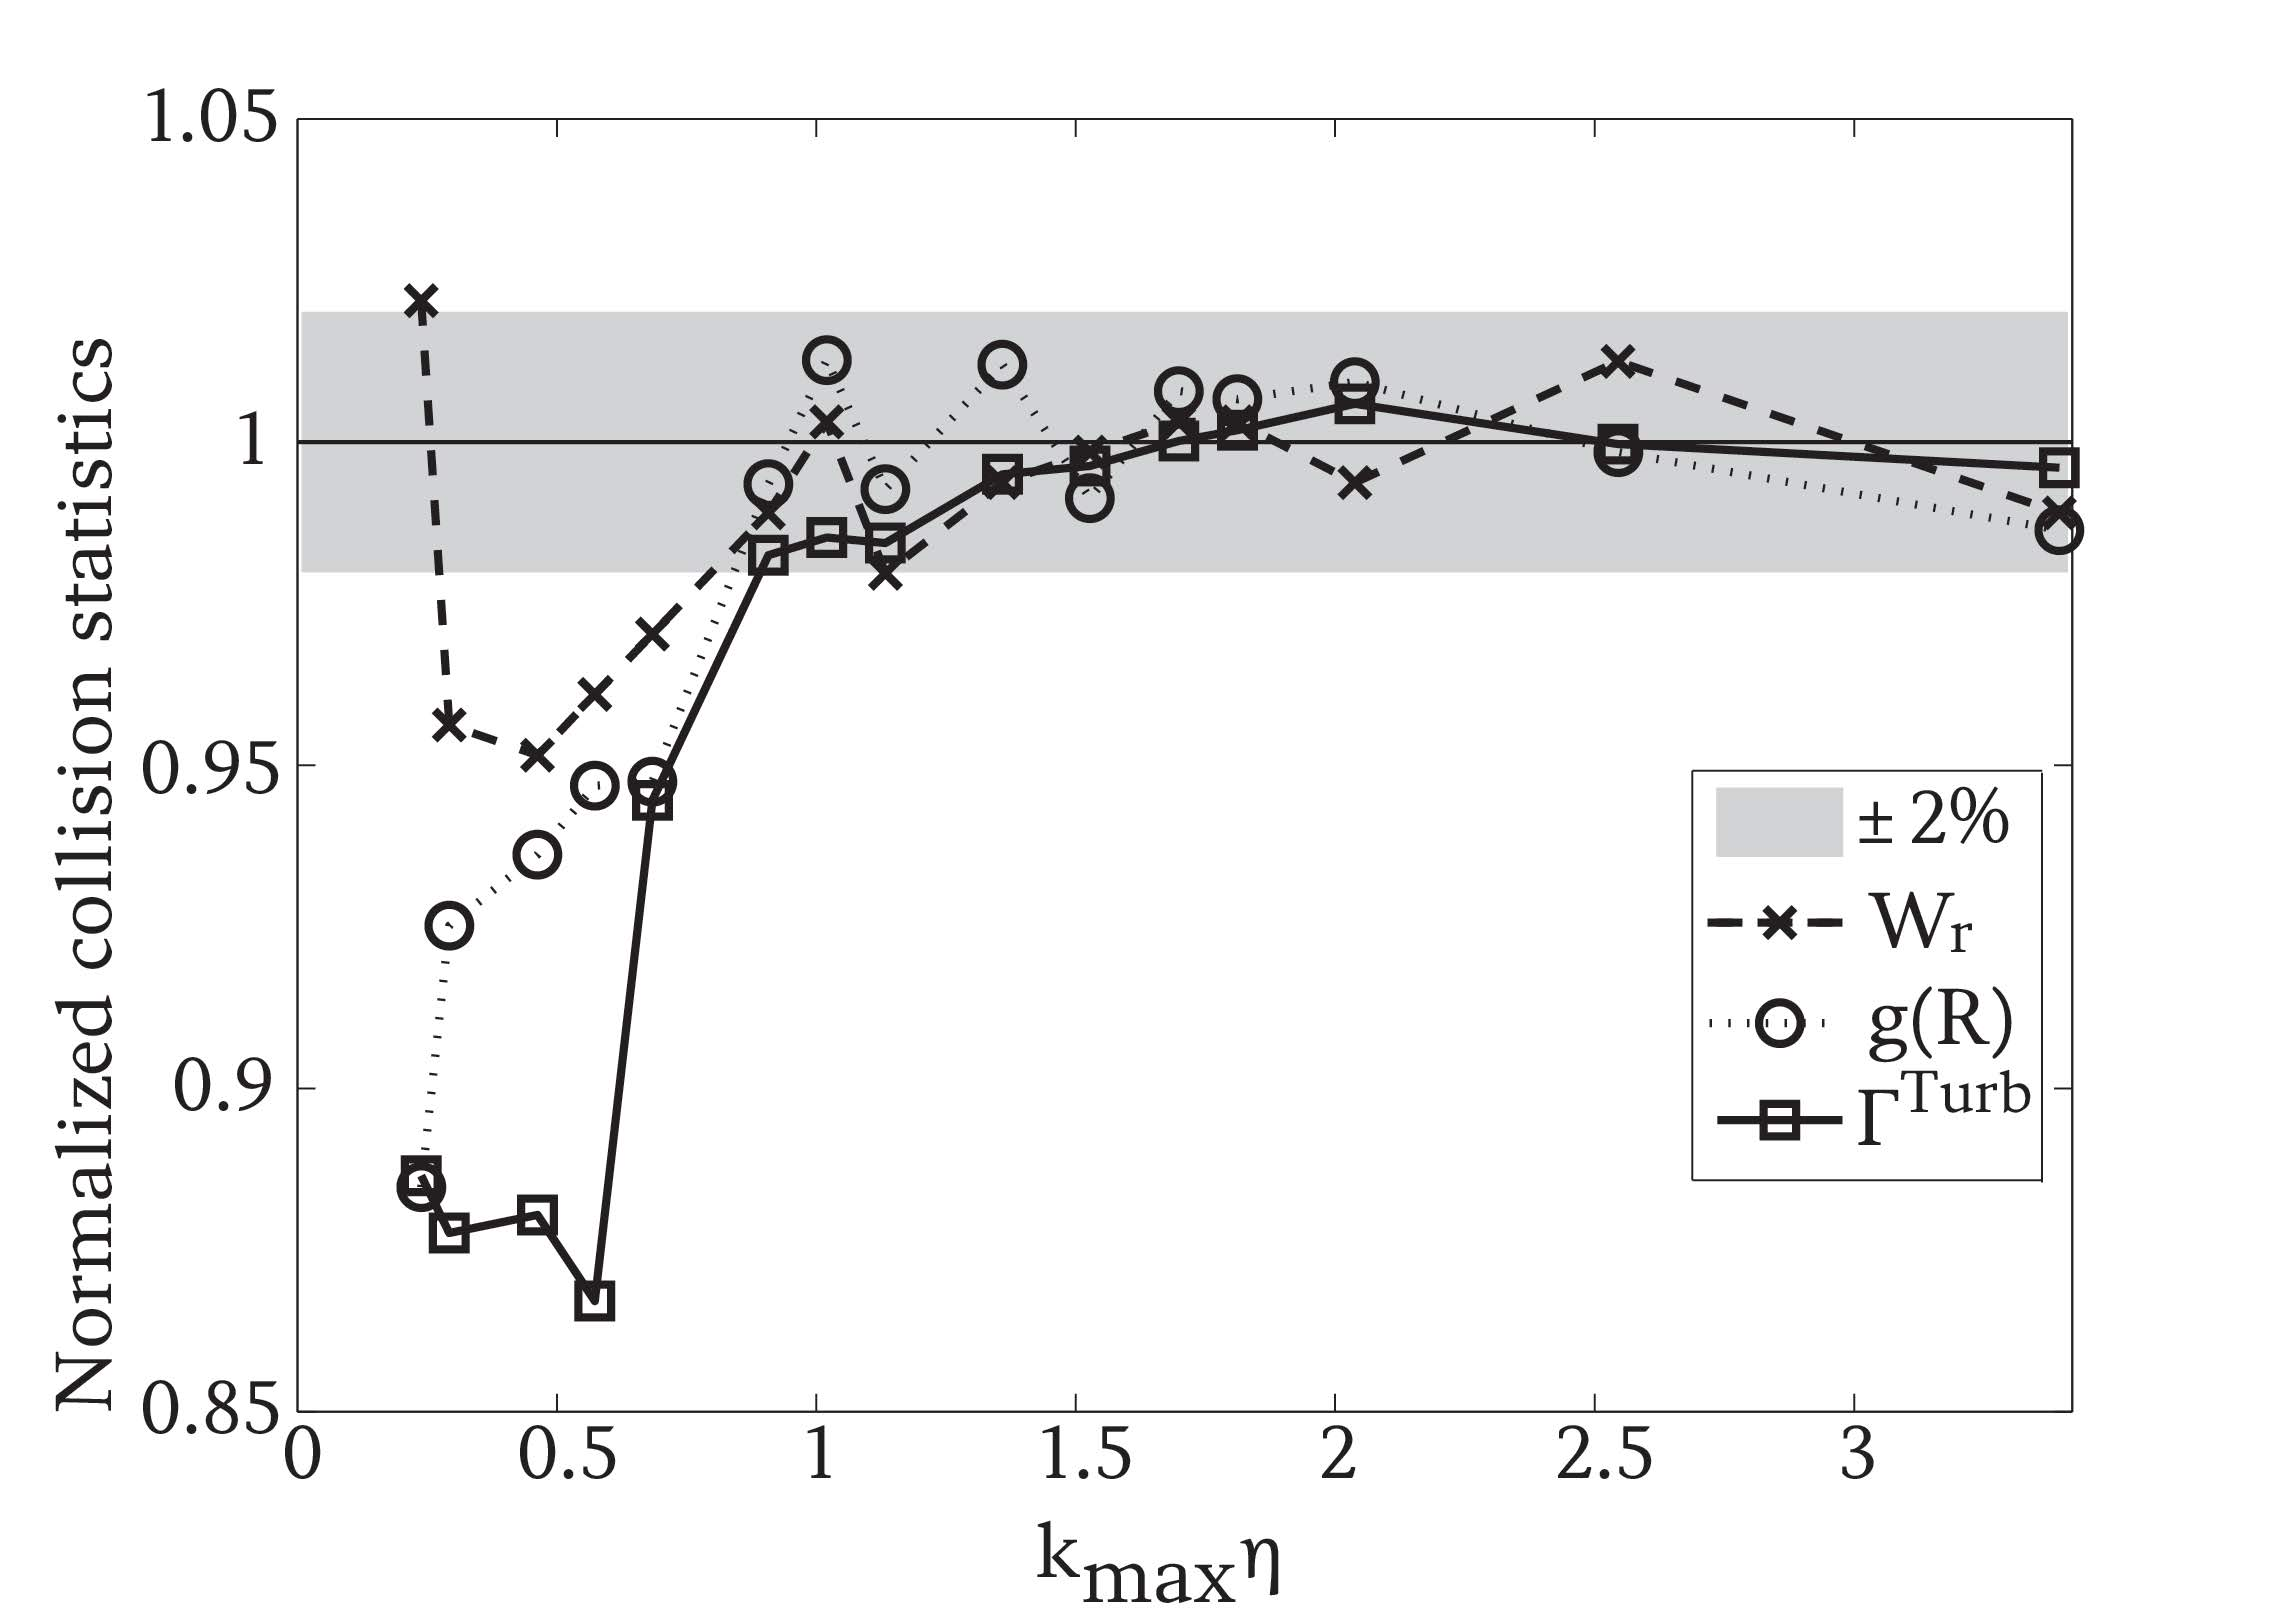
\includegraphics[width=\textwidth]{Figures/Chap2/kmaxeta.jpg} 
\caption{Collision statistics as a function of $k_{max}\eta$. All values are normalized by their respective average after $k_{max}\eta>1$. }\label{fig:kmaxeta1}
\end{figure}

To test the scalability of the code, we performed seven groups of simulations with different numbers of processors (2, 4, 8, 16, 32, 64, 128) on two different machines: The SGI Altix 4700 supercomputer at the University of Montreal and the Mammouth-parallel II machine at the University of Sherbrooke. Each group contained three members and we took the average of the three as a reference walltime. All tests were performed at $N = 256^3$ with $L=0.2$ m and we injected a total of $424,448$ droplets into the flow, half of which have a radius of 10 $\mu m$ and the other half with 20 $\mu m$. The code scales reasonably well on both machines. According to Amdahl's law, the performance of a parallelized program is constrained by its sequential part when number of processors increases \citep{Amdahl1967}. If the code is fully parallelized, the true walltime ($T_w$) will be half when number of processors ($N_p$) doubles. In other words, their relation can be precisely described by a power law formula with the power equals -1: $T_w=T_s\times N_p^{-1}$. Here $T_s$ is the walltime when the program is executed with single processor. The walltimes of our executions spanned from 60 minutes (with 128 processors) up to 2000 minutes (with 2 processors) on the SGI Altix, fitted into the curve of $T_w=3976$ (min) $\times N_p^{-0.8783}$. The experiments on the mp2 gave a fitted curve of $T_w=2433$ (min) $\times N_p^{-0.702}$. Even though we did not attain perfect scalability on both machines, we saw a significant speed-up of the simulations as the number of processors doubled. 

\subsubsection{Improvements in computing statistics of flow parameters} \label{sec:ch2_flowpara}

In this paper we used different approaches to obtain the EDR, the Taylor micro-scale ($\lambda$), and the $R_\lambda$ of the flow field. \citet{Franklin2005} estimated EDR from the energy spectrum, while we calculated it from the numerical integration of enstrophy ($\epsilon = 2\nu Z$, where Z is the total enstrophy), which provides more accurate values. $\lambda$ was calculated via $\sqrt{\frac{KE}{Z}}$ in \citet{Franklin2005}, where $KE$ is the total kinetic energy in the system, and our $\lambda$ was from $\sqrt{\frac{15\nu u\prime^2}{\epsilon}}$. Here $u\prime=\sqrt{\frac{2(KE)}{3}}$. $R_\lambda$ in our study was computed via $\frac{u\prime\lambda }{\nu}$, while $R_\lambda = \frac{\lambda\sqrt{2(KE)} }{\nu}$ in \citet{Franklin2005}.  Of course, these quantities respect the same scaling in Kolmogorov phenomenology, but not with the same proportionality constants. 

To quantify the difference in the resulting flow statistics, we re-ran the four cases in \citet{Franklin2005}. The results are listed in table \ref{tab:comp1} along with the \citet{Franklin2005} results for comparison. N is the number of grid points, ke is the initial KE. Flow statistics show that $\lambda$ in our study was around 3.0 times the value in \citet{Franklin2005} and $R_\lambda$ around 1.85 times. Since we did not change the actual properties of the flow but only the method of evaluating these statistics, similar collision statistics were expected under the same particle tracking and collision detection techniques. Indeed, the collision statistics in table \ref{tab:comp1} show that our results were indeed close to those of \citet{Franklin2005}, within a difference of $11\%$.


\begin{sidewaystable}
\begin{center}
\def\arraystretch{1.5}
\caption{Statistical parameters of the turbulent flow fields and corresponding collision statistics of four simulations from our study and from \citet{Franklin2005} (denoted as F05)\strut} \label{tab:comp1}
\begin{tabular}{ccccccccc}
\hline\hline
 N & \multicolumn{2}{c}{ $80^3$} & \multicolumn{2}{c}{$120^3$} & \multicolumn{2}{c}{$180^3$} & \multicolumn{2}{c}{$240^3$} \\
\hline
 model & DNS-MPI  & F05 & DNS-MPI &  F05  & DNS-MPI & F05 & DNS-MPI & F05 \\
\hline 
\multicolumn{9}{c}{Statistical parameters of the turbulent flow fields}\\

$\epsilon$(cm$^2$ s$^{-3}$) & 155 & 95 & 544 & 280 & 1371 & 656 & 2710 & 1535 \\ 

$\lambda$ (cm) & 1.10 & 0.35 & 0.90 & 0.29 & 0.78 & 0.26 & 0.70 & 0.23 \\ 
 
$R_\lambda$ & 60 & 33 & 76 & 40 & 89 & 48 & 102 & 55 \\ 

$u\prime$(cm s$^{-1}$)& 9 & 9 & 13 & 12 & 18 & 16 & 23 & 21 \\ 

$k_{max}\eta$ & 1.8 & 1.8 & 2.0 & 2.1 & 2.4 & 2.6 & 2.7 & 2.7 \\ 
 
$\eta (cm)$ & 0.07 & 0.07 & 0.05 & 0.06 & 0.04 & 0.05 & 0.04 & 0.04 \\ 
\hline
\multicolumn{9}{c}{Collision statistics}\\

$\Gamma \times10^{10}$ ($m^3 s^{-1}$)  &   $1.1267$  & $1.1054$ & $1.2940$  & $1.2420$  & $1.6629$ & $1.4960$  & $2.2736$ &  $2.1748$ \\ 

$g(R)$ & $1.0779$ & $1.0825$  & $1.1329$  & $1.1621$ & $1.2847$  & $1.2432$ & $1.4720$ & $1.4183$  \\ 
$\mathbf{W_r}$ (cm s$^{-1}$) & $1.85$  &  $1.8650$  &  $2.00$  & $2.1248$  & $2.26$   & $2.1248$  & $2.76$ & $2.7518$ \\

\hline 
\end{tabular} 
\end{center}
\end{sidewaystable}

\subsubsection{Separating the effects of $R_\lambda$ and EDR} \label{sec:ch2_separate}

As explained in section \ref{sec:ch2_intro}, the conclusions regarding $R_\lambda$ from \citet{Franklin2005} needs further exploration since the effects of EDR and $R_\lambda$ cannot be separated. To solve this problem we fix $\Delta x$ when simulating the same EDR, since EDR is determined by $\Delta x$ alone when $k_{max}\eta$ is fixed (See section \ref{sec:ch2_compares}). To increase $R_\lambda$, we increase the number of grid points (N) and hence the computational domain size (L), thereby resolving larger scales of the flow while keeping EDR fixed. Since $\Delta x$ in our study is linearly proportional to $\eta$ and $R_\lambda$ scales with domain size, L, it follows that $N \equiv L/\Delta x \propto L/\eta \propto (R_\lambda)^{3/2}$. Therefore, when varying $R_\lambda$ at fixed EDR, we changed N and fixed $\Delta x$. Likewise, when varying EDR to study its influence, we tuned $\Delta x$ to obtain our fixed value $k_{max} \eta=1.3$ and fixed N. 

\subsubsection{Two forcing schemes}\label{sec:ch2_forcing}

The total kinetic energy in the forcing band is fixed in \citet{Franklin2005}. We refer to this forcing scheme as forcing1. However, not knowing how much kinetic energy should be fixed to reach a desired average EDR, we have to manually adjust the initial energy in the forced waveband by trial and error, which is very inefficient. For this reason, we propose a modified version of the forcing (termed forcing2), which injects equal amounts of energy into the forcing band at each time step. The energy supply at the forcing scales is balanced by dissipation at the viscous scales when turbulence reaches statistical stationarity. It follows that the rate of energy injection can  easily be determined by the EDR at the initial time step and held constant thereafter. In this way, we decrease the amount of computations by specifying a steady average EDR directly.

To test the accuracy and efficiency of forcing2, we reran the simulation of \citet{Franklin2005} at $N=80^3$ with this forcing and compared the results with those from forcing1. The EDR for forcing1 was 155 $cm^2s^{-3}$ (see table \ref{tab:comp1}). We used this value to calculate the energy injection rate in the case of forcing2. Since the turbulence is both statistically stationary and ergodic, ensemble averages can be represented by time averaging.  Figure \ref{fig:specs} (a) demonstrates that forcing2 reproduced a very similar ensemble kinetic energy spectrum as forcing1 with a negligible difference of about 2\% in flow properties. This result demonstrates that forcing2 produces reliable results that are statistically identical to forcing1, but arrives at the kinetic energy spectrum, obtained by specifying the EDR, much more readily. To examine further the efficiency and accuracy of forcing2, we did another four simulations with $\epsilon \approx 1000 cm^2 s^{-3}$. The computational box size was fixed but resolution was different in each case. Figure \ref{fig:specs} (b) illustrates that the ensemble kinetic energy spectra from different resolutions lay on top of each other without any discernible shifts. This result lends support to the capability of forcing2 to produce precise mean EDR covering a range of spatial resolutions, since DNS average EDRs vary within only $\pm 1\%$. Although forcing2 is more efficient in controlling the average EDR than forcing1, most of our computations were obtained using forcing1. To avoid repeating the costly calculations our statistics will be analyzed from these data, bearing in mind that the EDRs show scatter within $\pm15\%$ from the desired value, but there were only two cases with scatter beyond $\pm10\%$. Forcing2 was used for the validation tests only.

\begin{figure}[ht]
\centering
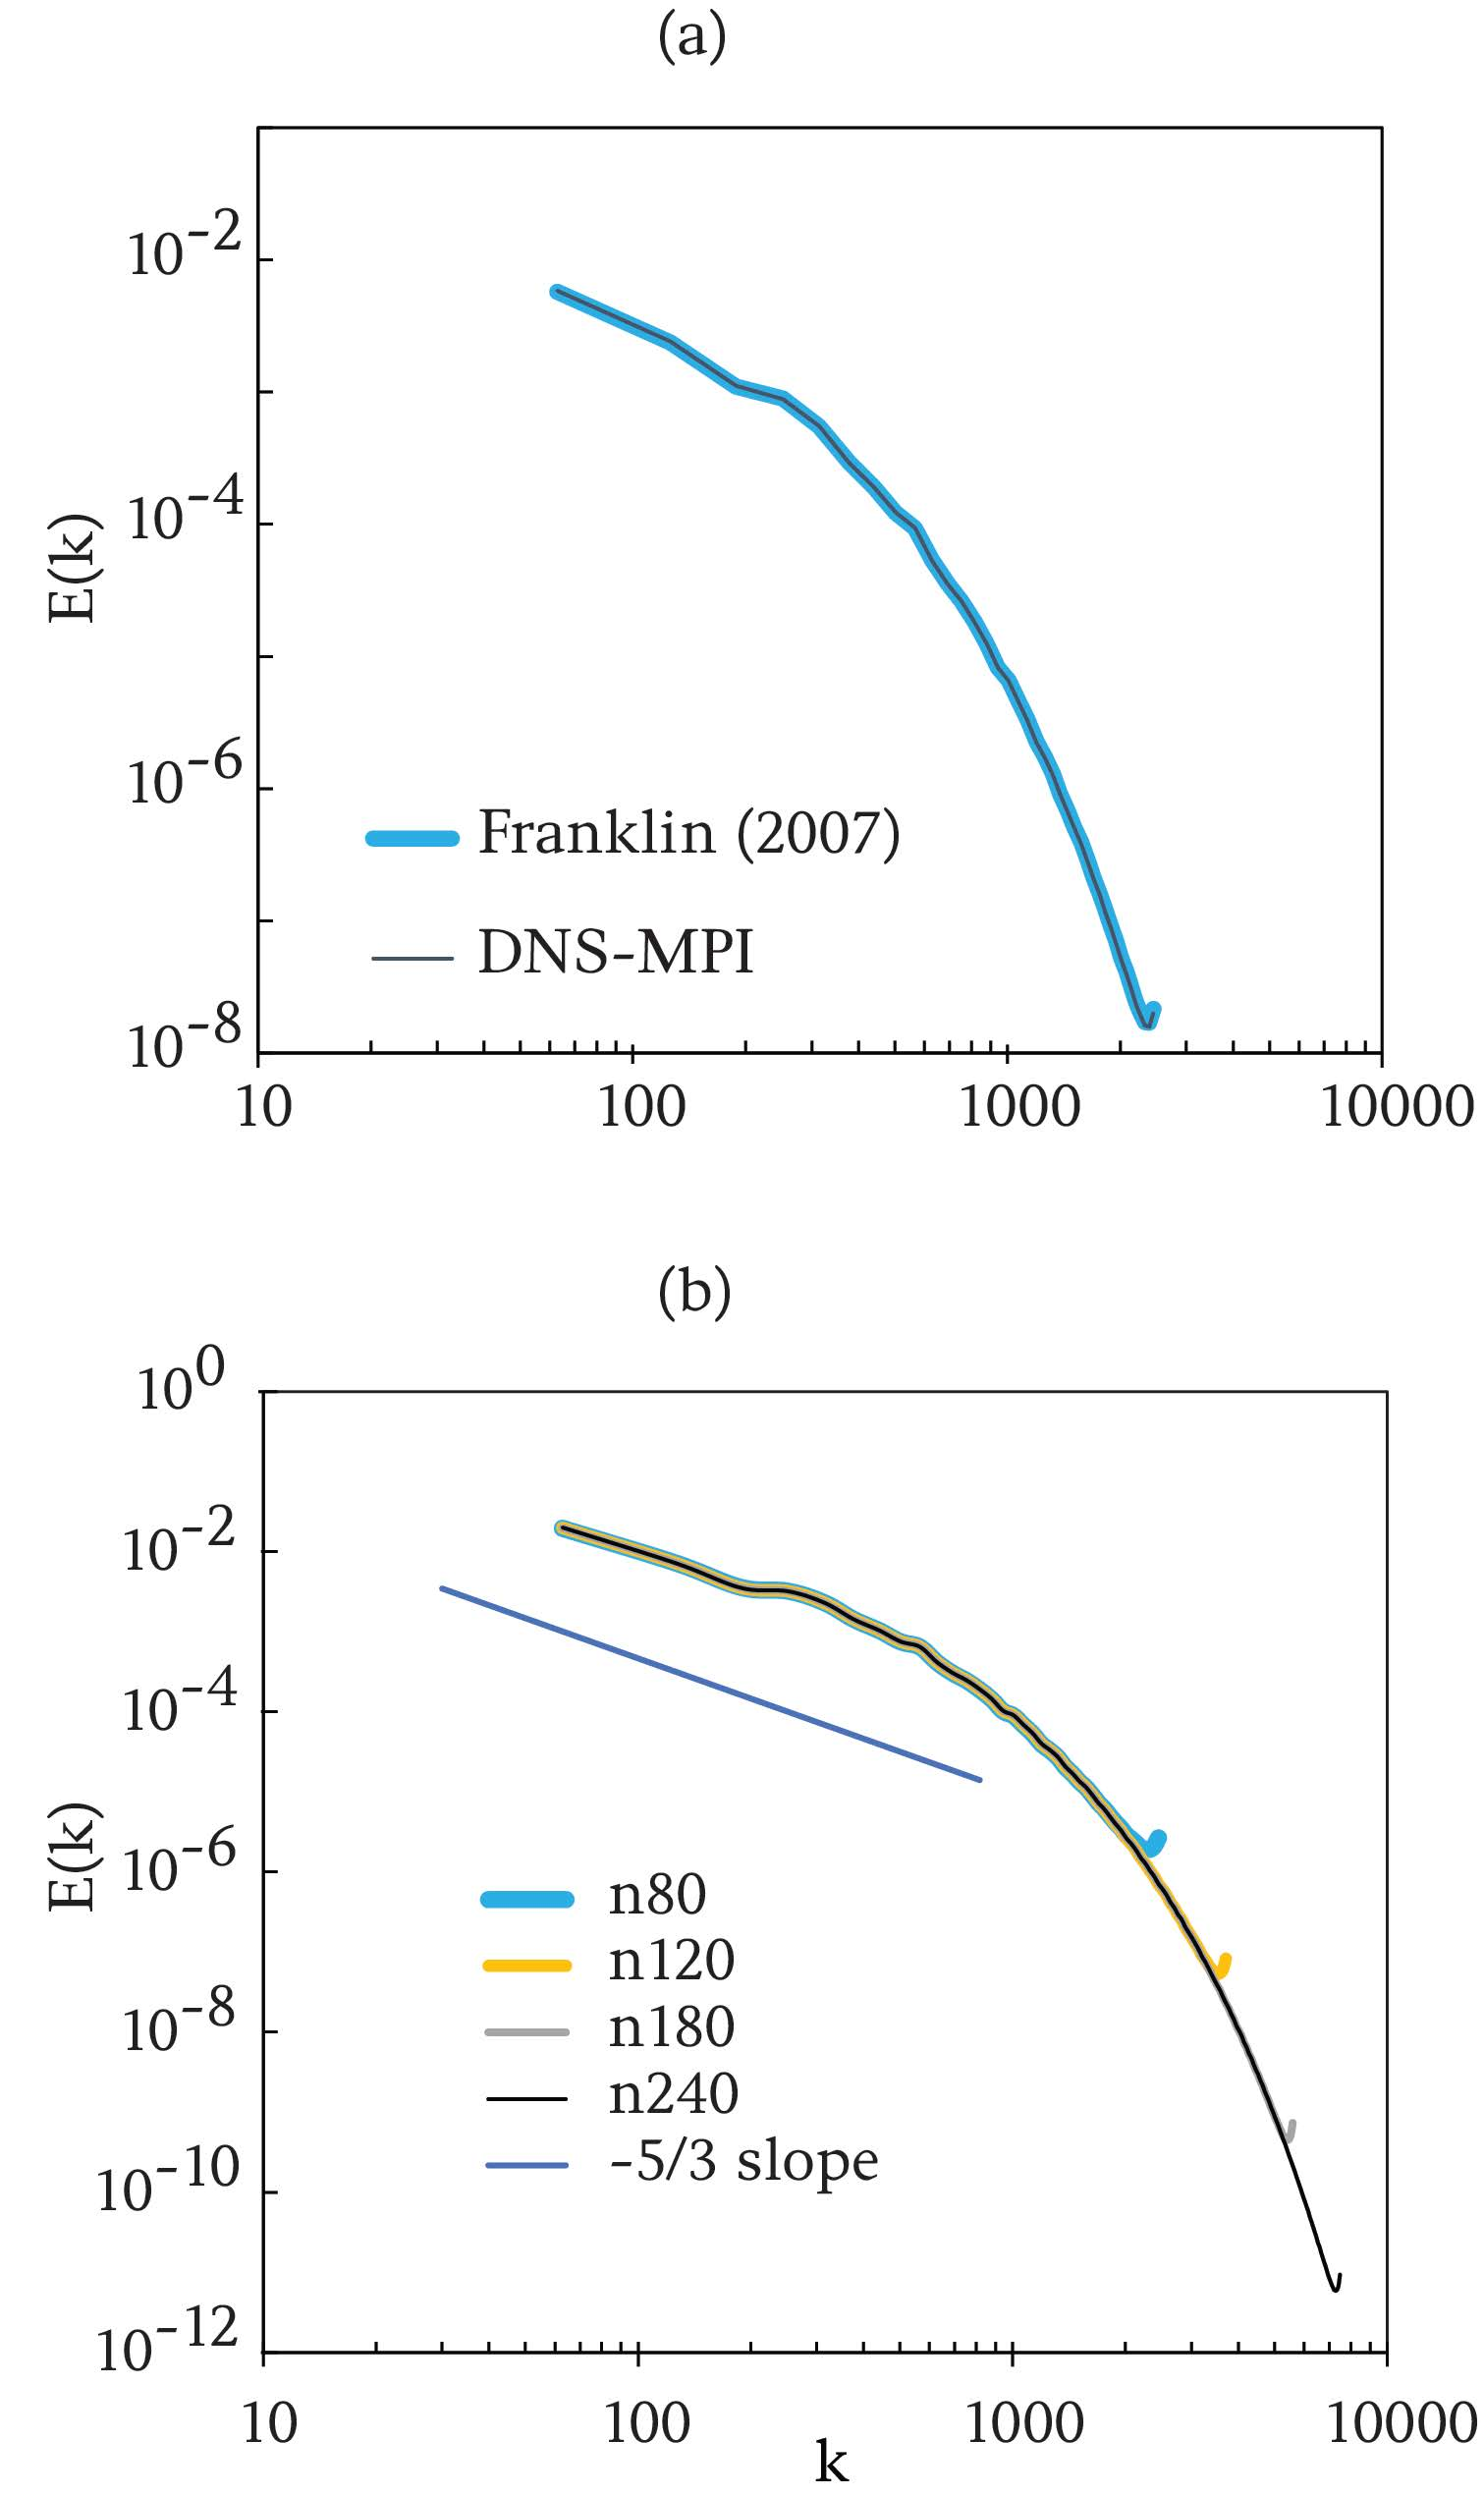
\includegraphics[width=0.7\textwidth]{Figures/Chap2/specs.jpg}
\caption{(a) Ensemble energy spectra from \citet{Franklin2007}'s forcing scheme (thick blue line) and from forcing2 (thin black line) with $\epsilon \approx$ 155 $cm^2s^{-3}$ and (b) ensemble energy spectra from forcing2 at four different resolutions with $\epsilon \approx 1000$ $cm^2 s^{-3}$, the domain width is fixed to 0.1 m in three directions for all simulations} \label{fig:specs}
\end{figure}

\section{Results} \label{sec:ch2_result}

To test the $R_\lambda$-dependency and EDR-dependency, our simulations employed five different eddy dissipation rates ($\epsilon = $ 50, 200, 500, 1000 and 1500 $cm^2s^{-3}$), and nine different box sizes ($N = 64^3, 96^3, 128^3, 192^3, 256^3, 384^3, 512^3$ and $1024^3$). We managed to run most of the scenarios except those with both high resolution and low dissipation rates (See figure \ref{fig:perform}). The reason is that N is largest in the highest resolution simulation and $\Delta x$ is largest at the lowest EDR run (see section \ref{sec:ch2_mpi})). As a consequence, the slab volume and the number of droplets assigned to each processor become very large, causing an inordinate amount of communication between processors yielding extremely slow computations. Nevertheless, the successful runs were sufficient for us to quantify the turbulence effects on droplet collisions as they span a broad range of EDR and $R_\lambda$.

\begin{figure}[ht]
\centering
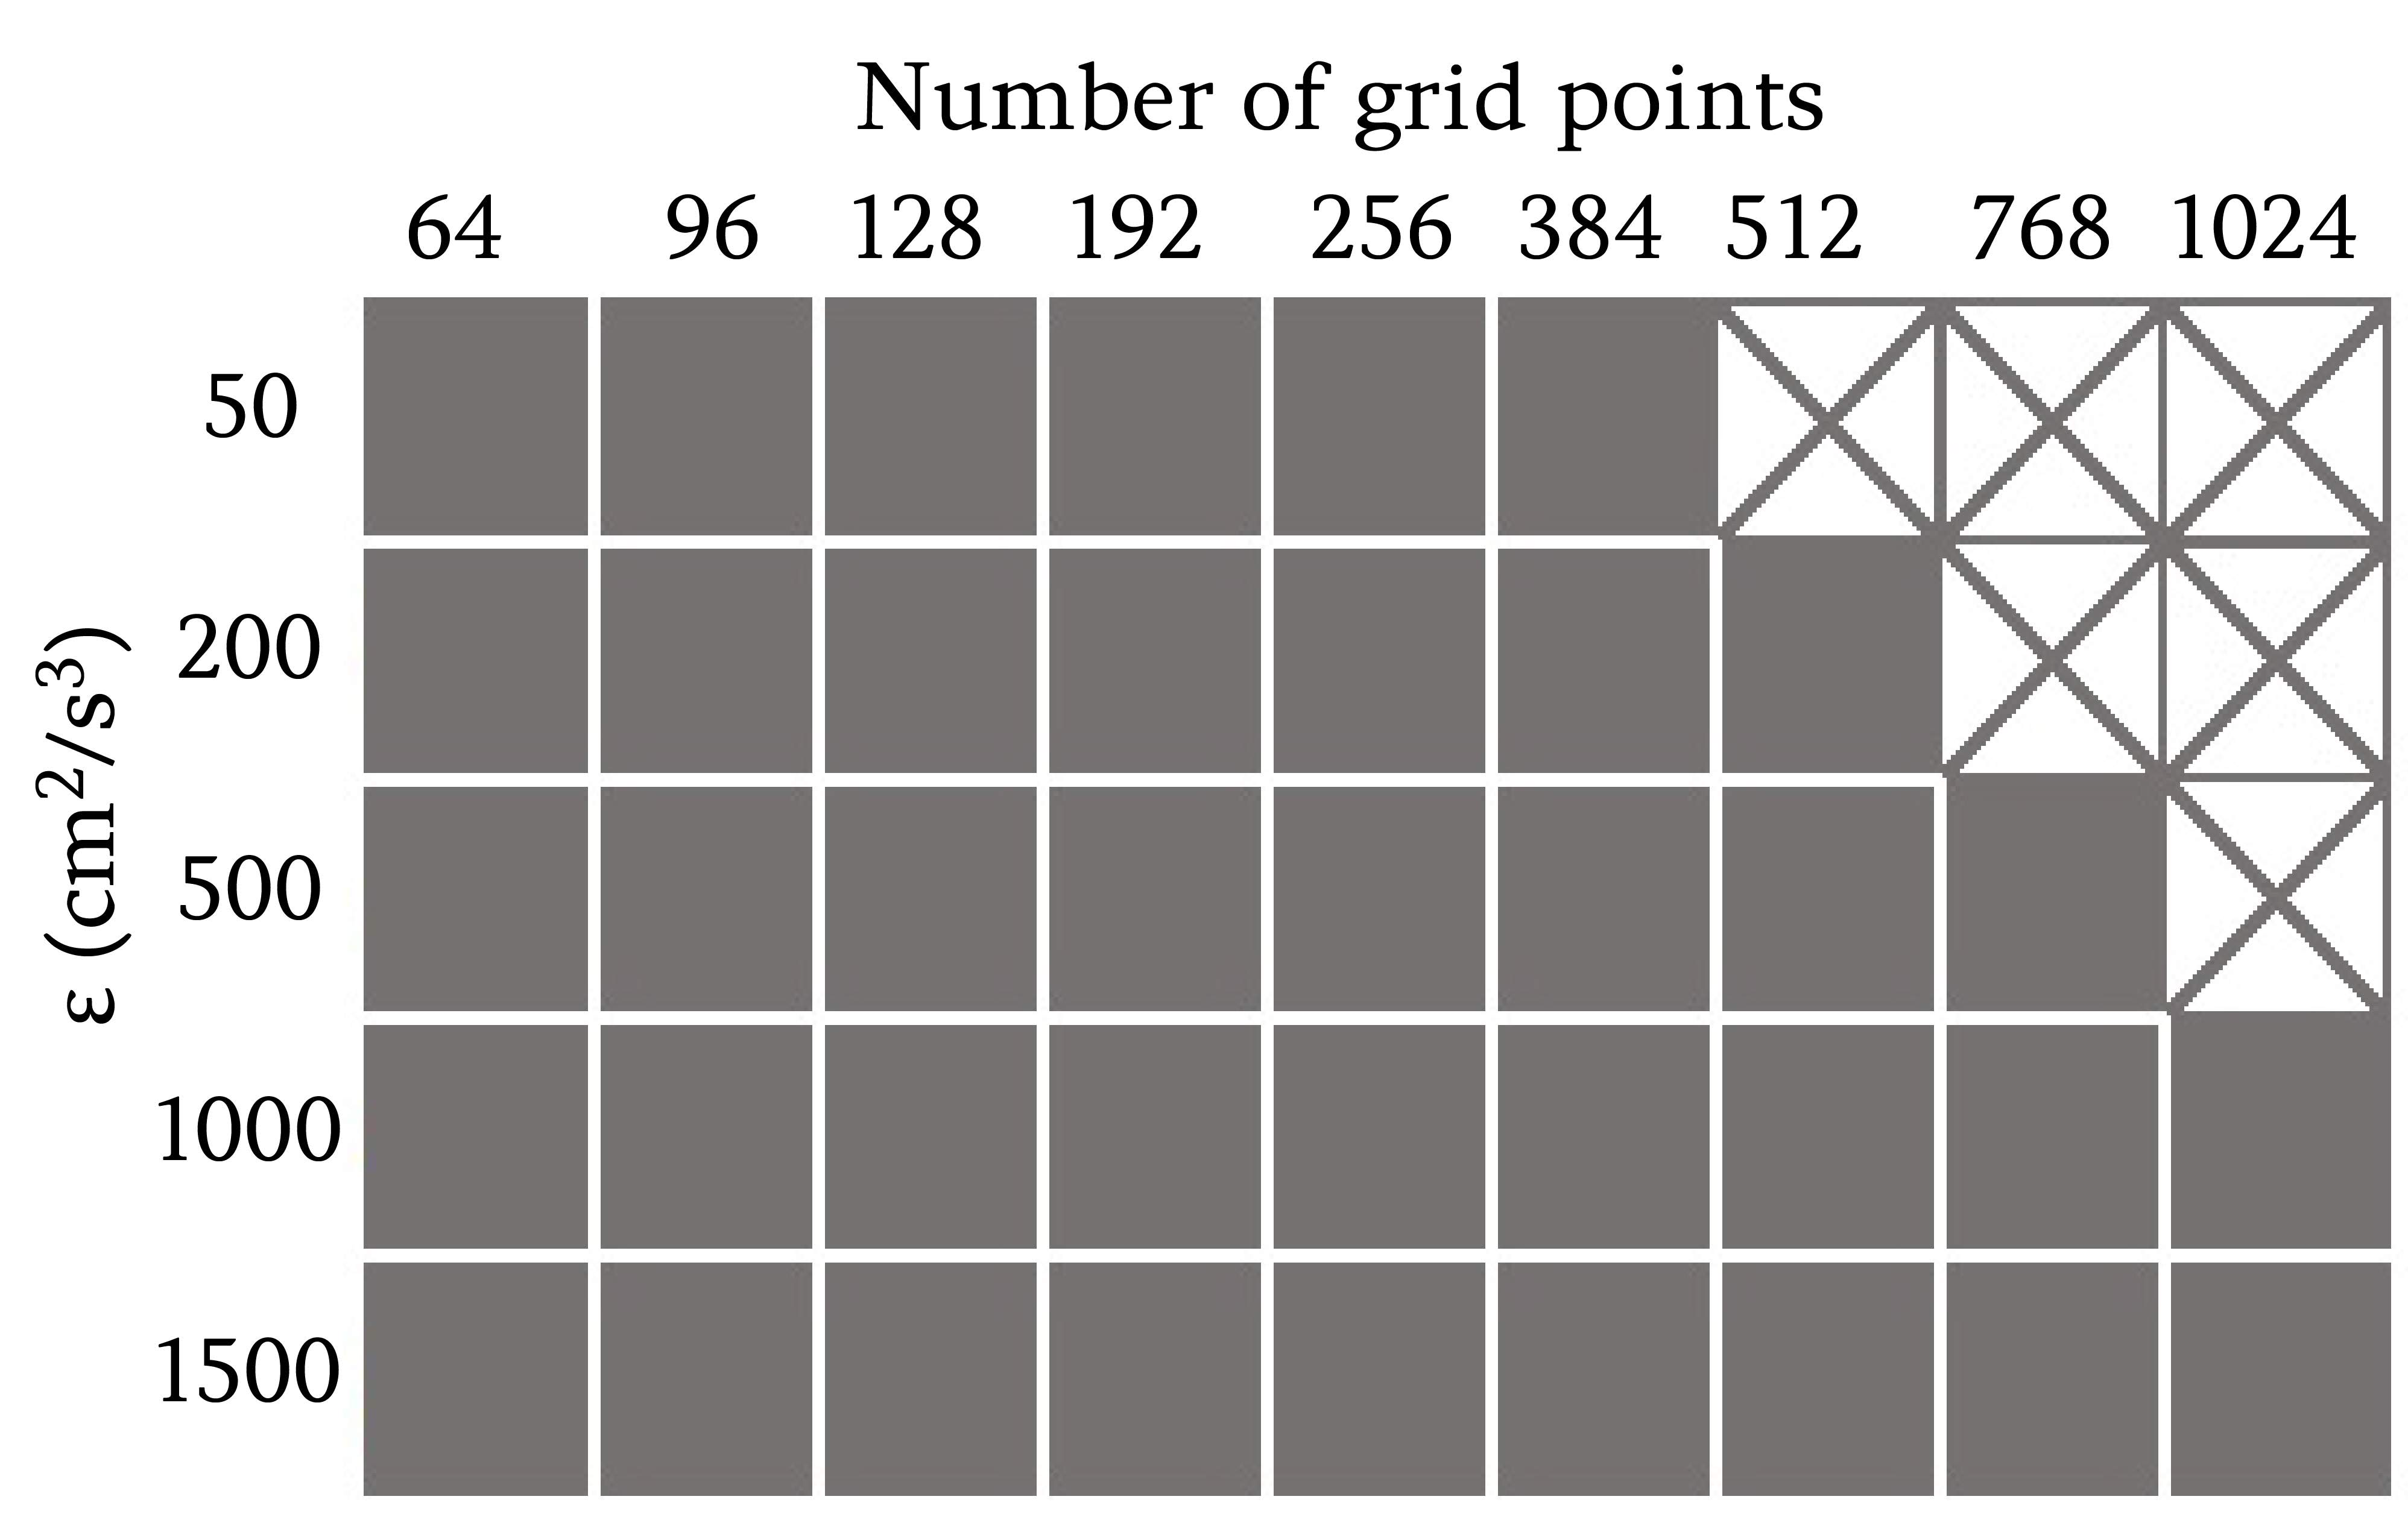
\includegraphics[width=0.8\textwidth]{Figures/Chap2/perform.jpg}
\caption {Overview of performed simulations over different $R_\lambda$-values and EDRs. Successful runs are shaded with gray, failed runs are marked by "$\times$"} \label{fig:perform}
\end{figure}


\subsection{Collision statistics with different box sizes ($R_\lambda$)} \label{sec:ch2_re}

The $R_\lambda$ in our simulations ranged from $63$ ($N=64^3$) to $589$ ($N=1024^3$), which gave us a good indication of how collision statistics depend on $R_\lambda$ or equivalently on the box size. \citet{Rosa2013} tested the convergence of collision statistics of 20-20 $\mu m$ droplet pairs and 30-30 $\mu m$ pairs with $R_\lambda$ using two different forcing schemes: one was stochastic forcing, where random acceleration was added to the velocity component in a low wave-number band, and the other was deterministic forcing in which the energy level in the two smallest wavenumber bands was fixed. They concluded that the RDF between large droplets ($r=30$ $\mu$m) were harder to converge with $R_\lambda$ than between small droplets ($r=20$ $\mu m$) because they were under the influence of larger scales of motion. The growing trend at low $R_\lambda$ in both forcings, as explained in their paper, was because more collision-related scales were resolved when $R_\lambda$ increased until a saturation level was reached. In addition, there was another possible contribution. Although the average dissipation rate was set to 400 $cm^2 s^{-3}$ in all cases, some variations were observed. The curves of RDFs follow closely the fluctuations of average EDR in both forcing schemes. Under stochastic forcing the EDR increased slightly with $R_\lambda$ \citep[see section 4.1 and figure 2 in][]{Rosa2013} while the corresponding RDFs were larger as well (see figure 15 in their paper). Under deterministic forcing the EDR reached its peak around $R_\lambda \approx 100-200$ and a similar pattern was also found in the RDFs at $r=30$ $\mu m$. 
According to our DNS, the sensitivity of the RDF of 25-25 $\mu m$ droplets to EDR (i.e., $\frac{\Delta g(R)}{\Delta \epsilon}$) was about $1.42 \times 10^{-2}$ $(cm^2 s^{-3})^{-1}$ for EDR around $500$ $cm^2 s^{-3}$, i.e., increasing $1 cm^2 s^{-3}$ in EDR will result in an increase of $1.42 \times 10^{-2}$ in g(R). This implies that a change of $100$ $cm^2s^{-3}$ in EDR will result in a change of 1.42 in the value of RDF, which is of the same order of magnitude as that of the RDF fluctuations in their large $R_\lambda$ regions. In section \ref{sec:ch2_diss}, we will show in detail that collision statistics are very sensitive to the EDR. 


We are in a position to compare the collision statistics with a wider range of $R_\lambda$ under fixed EDRs. Figure \ref{fig:Re_ck} demonstrates the collision kernel between 10 $\mu m$ droplets and 20 $\mu m$ droplets with different $R_\lambda$, with each curve indicating different EDRs when using forcing 1. The curves fluctuate mainly because the mean EDR in each run scattered within 15\% from the nominal value shown in the legend. The standard deviation of the statistics increases with $R_\lambda$, which can be induced by the intensified intermittency of the turbulence as domain size increases. \citet{Kolmogorov1962} conjectured that the variance of local (instantaneous) dissipation rate, $\epsilon\prime$, normalized by its square mean value scales with Reynolds number as follows: $\frac{\overline{\epsilon\prime^2}} {\overline{\epsilon\prime}^2} \sim \big(\frac{L}{\eta}\big)^\mu = R_\lambda^{\frac{3\mu}{2}}$, with the intermittent exponent $\mu = 0.25$ confirmed by later experiments and atmospheric observations \citep[e.g., ][]{Pope2000, Siebert2010}. Note that $\frac{\overline{\epsilon\prime^2 }} {\overline{\epsilon\prime}^2}$ is also the vorticity kurtosis K, and can be used to quantify the level of intermittency. We calculated K with different $R_\lambda$ at the EDR of $1000$ $cm^2s^{-3}$ and found our exponent consistent with $\mu=0.25$ with a relative error of 2.75\%. Though intermittency experienced a power law growth with the expansion of domain size, the collision kernel shown in figure \ref{fig:Re_ck} nevertheless is insensitive to $R_\lambda$, explicitly showing that the effect of intermittency is insignificant, at least over the simulated range. This flatness with $R_\lambda$ was also found in the collision kernel of all other droplet pairs including both same-sized collisions and cross-sized collisions as shown in panel A-B of figure \ref{fig:re_cs}. The standard deviation was of a similar order of magnitude as in figure \ref{fig:Re_ck} and therefore is not shown. The fluctuations in the curves were caused by slight variations in the dissipation rate, as mentioned earlier. As can be seen from the gray dashed line in panel A(ii), the EDR varied around $500$ $cm^2 s^{-3}$ over different simulations, creating a spike around $R_\lambda = 180$. This, as a consequence, diminished the flatness of these collision statistics. Panel B of the figure demonstrates the same fact with another dissipation rate. As for RDF and RRV shown in panel C and D respectively, the Reynolds number did not alter the collision statistics. Specifically, previous studies have shown that clustering happens in low-vorticity regions \citep[e.g., ][]{Maxey1987}. Therefore, we found it interesting that the RDF is also independent of domain size and we conclude that intermittency has a relatively small impact. However, this conclusion has to be interpreted cautiously. It is possible that the intermittency is still too weak, since the $R_\lambda$ here may not be sufficiently large to show the high levels expected in real cumulus clouds. The $R_\lambda$-independency implies that the large-scale motion has little effect on the droplets and the collision-related scales have been fully resolved at even small $R_\lambda$ ($\sim 60$). Droplets of small Stokes number adjust quickly to the local fluid acceleration before colliding with surrounding droplets and the local influence might greatly dominate over their acceleration history given by the large-scale motions. Thus, the effect, if any, of $R_\lambda$ on droplet collision statistics is secondary compared to the effects from the local dissipation rate and Stokes number. As discussed in section \ref{sec:ch2_intro}, the $R_\lambda$-dependency is in fact mainly the result of the model's inadequate flow scale separation seen only at very low resolutions, i.e., the failure to resolve all the collision-related scales is because the DNS box size is too small. Cloud systems are characterized by an enormous span of scales and their real Reynolds number is too large to be amenable to DNS. Thus the $R_\lambda$ calculated from DNS is determined by computational box size, L, rather than any real scale separation in clouds. The same conclusion can  apply to $u\prime$, following the scaling $u\prime = (\epsilon L)^{1/3}$. As a result, when interpreting the sensitivity of collision statistics to $R_\lambda$ from DNS data, we should be aware of the other quantities that are changing with the model configuration. We believe that the scale of turbulence affecting droplet collisions is on the order of the mean separation distance of cloud droplets. Generally, cloud droplet number concentration is on order of 10-1000 $cm^{-3}$, depending on the cloud type \citep[e.g., ][]{Twomey1959, Bennartz2007, Leaitch1992}. This gives an average droplet separation distance of the order of 0.1-1 mm, which is close to the order of the Kolmogorov length scale for the typical range of EDRs ($50-1500 cm^2s^{-3}$) in clouds. As long as the model resolves scales down to the droplet separation distance, which is far below our smallest computational domain size, $R_\lambda$ becomes irrelevant and the turbulence can be characterised by EDR alone. 


\begin{figure}[ht]
\centering
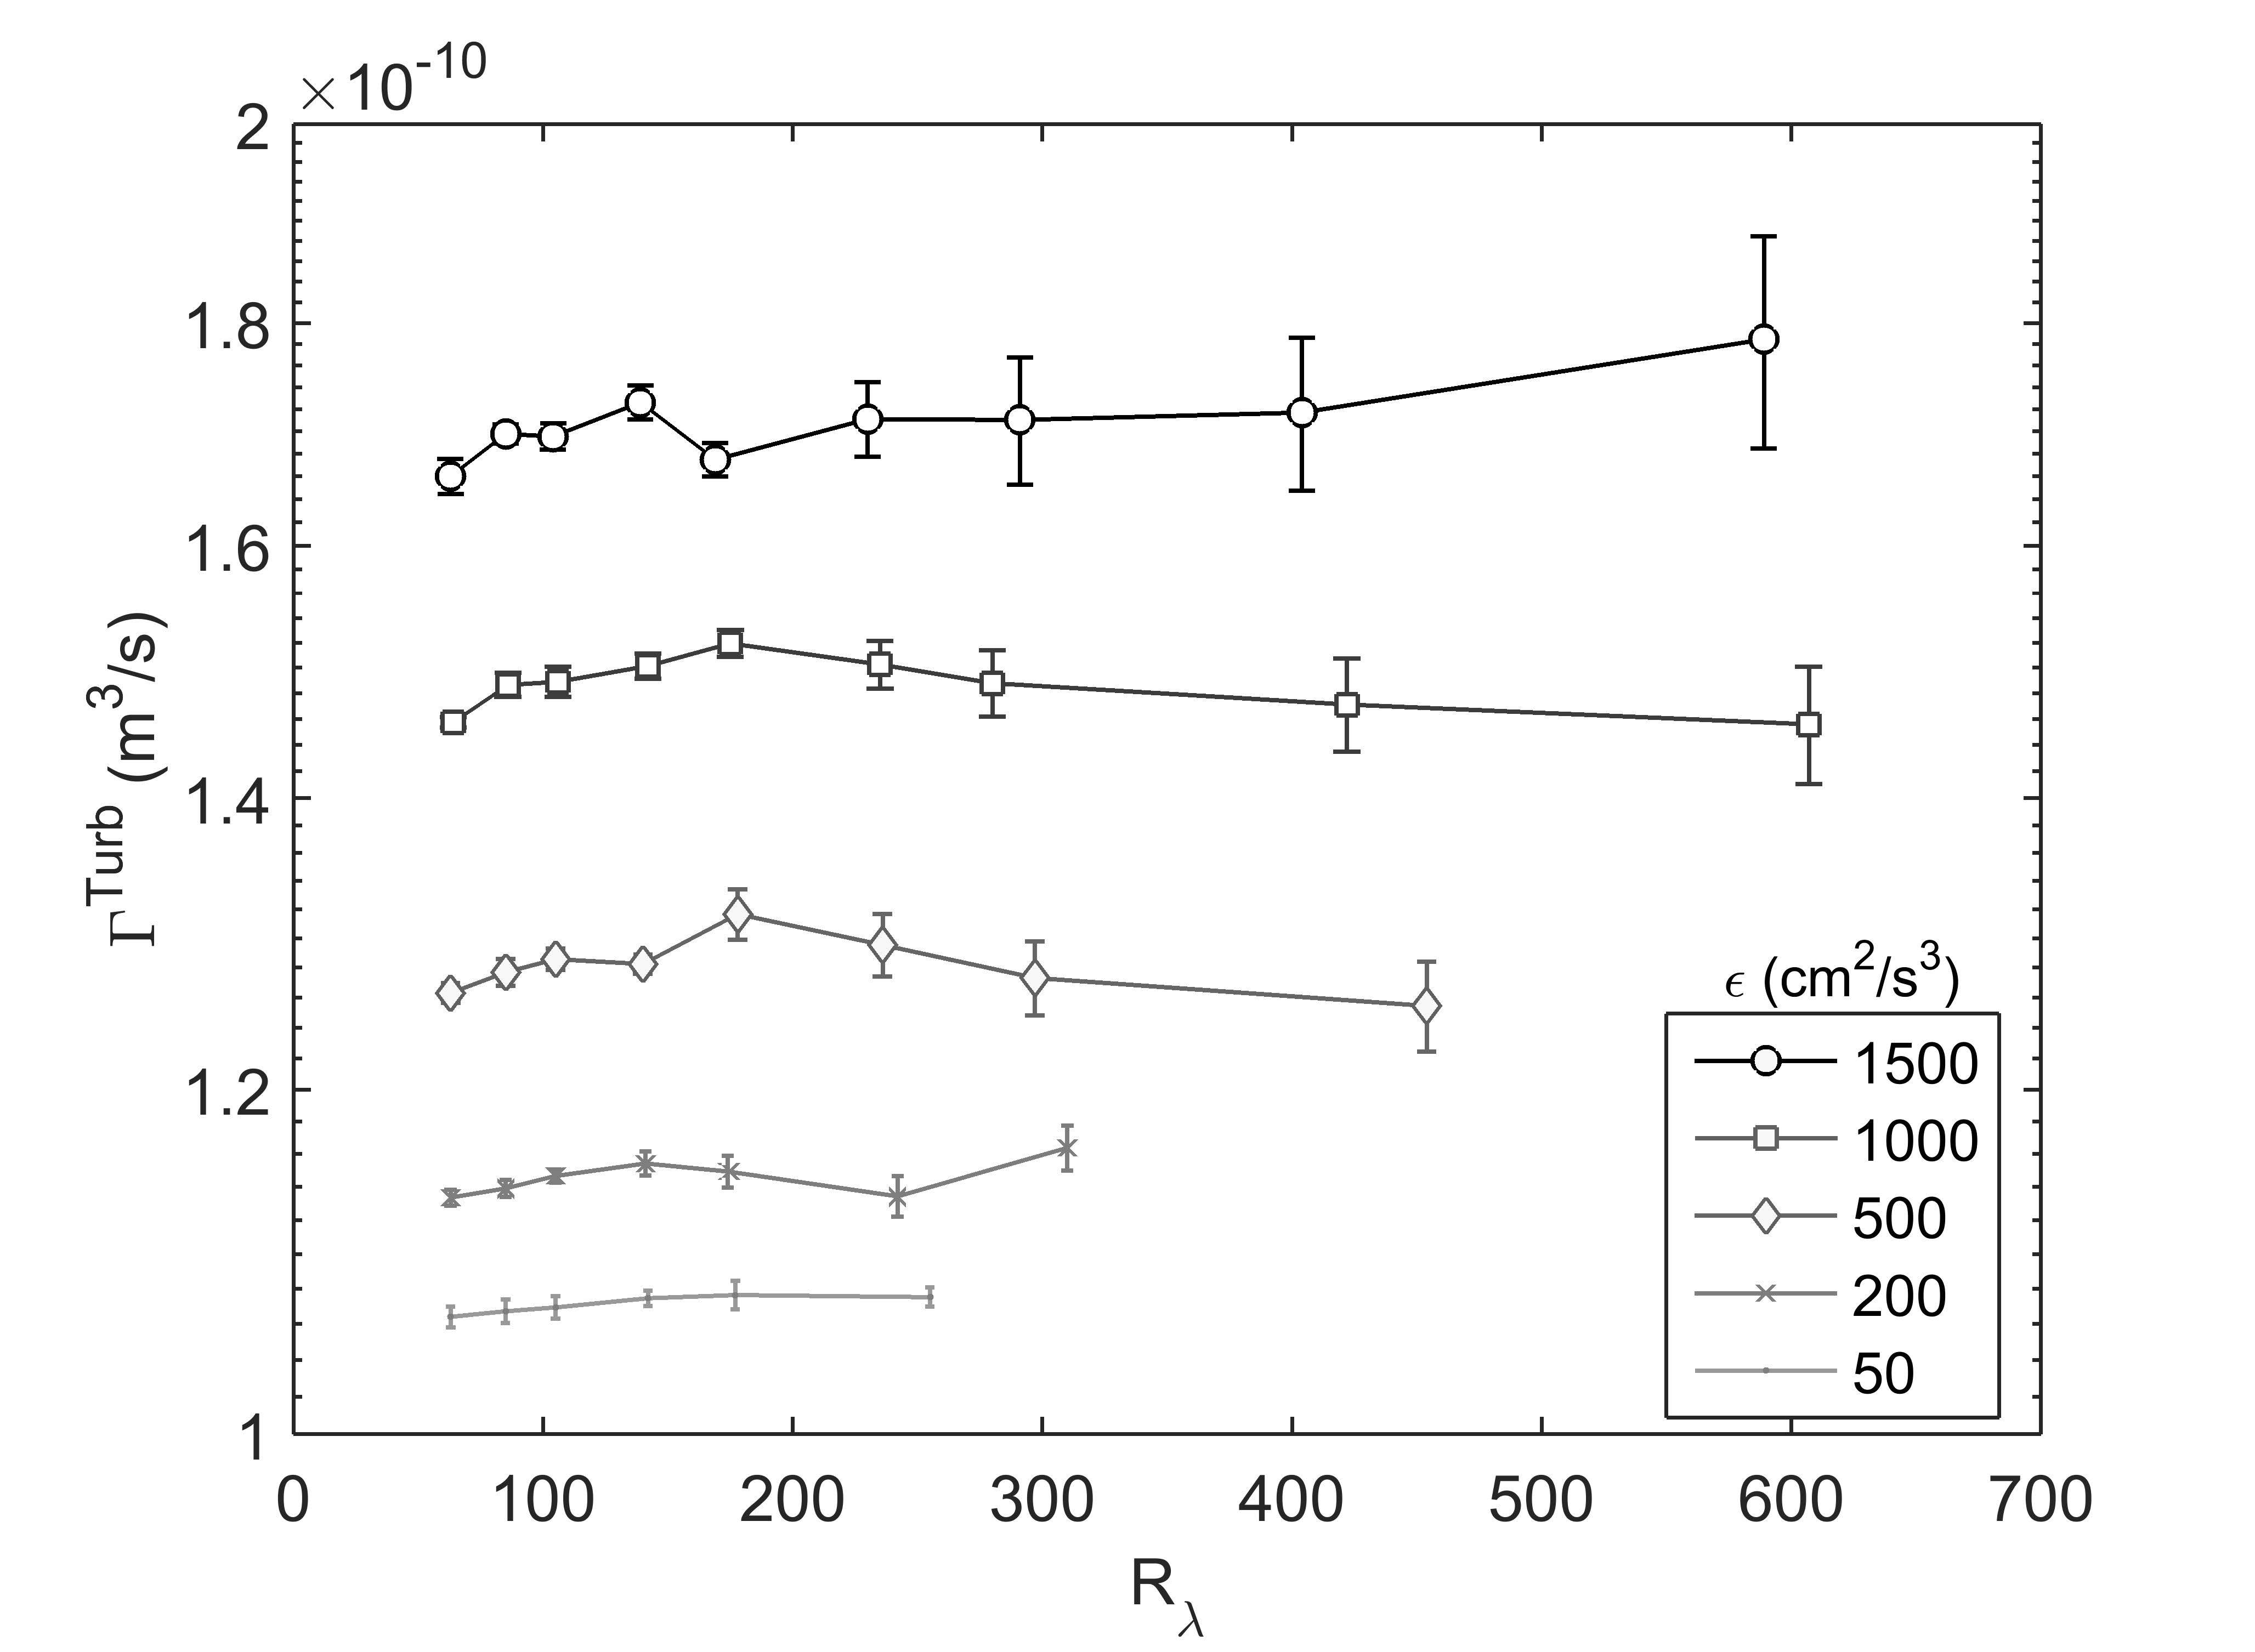
\includegraphics[width=0.8\textwidth]{Figures/Chap2/Re_ck.jpg}
\caption{Collision kernel of 10-20 $\mu$m collisions as a function of $R_\lambda$ with error bars representing one standard deviation. Values of EDR are represented by the grayscale.} \label{fig:Re_ck}
\end{figure}

\begin{figure}[ht]
\centering
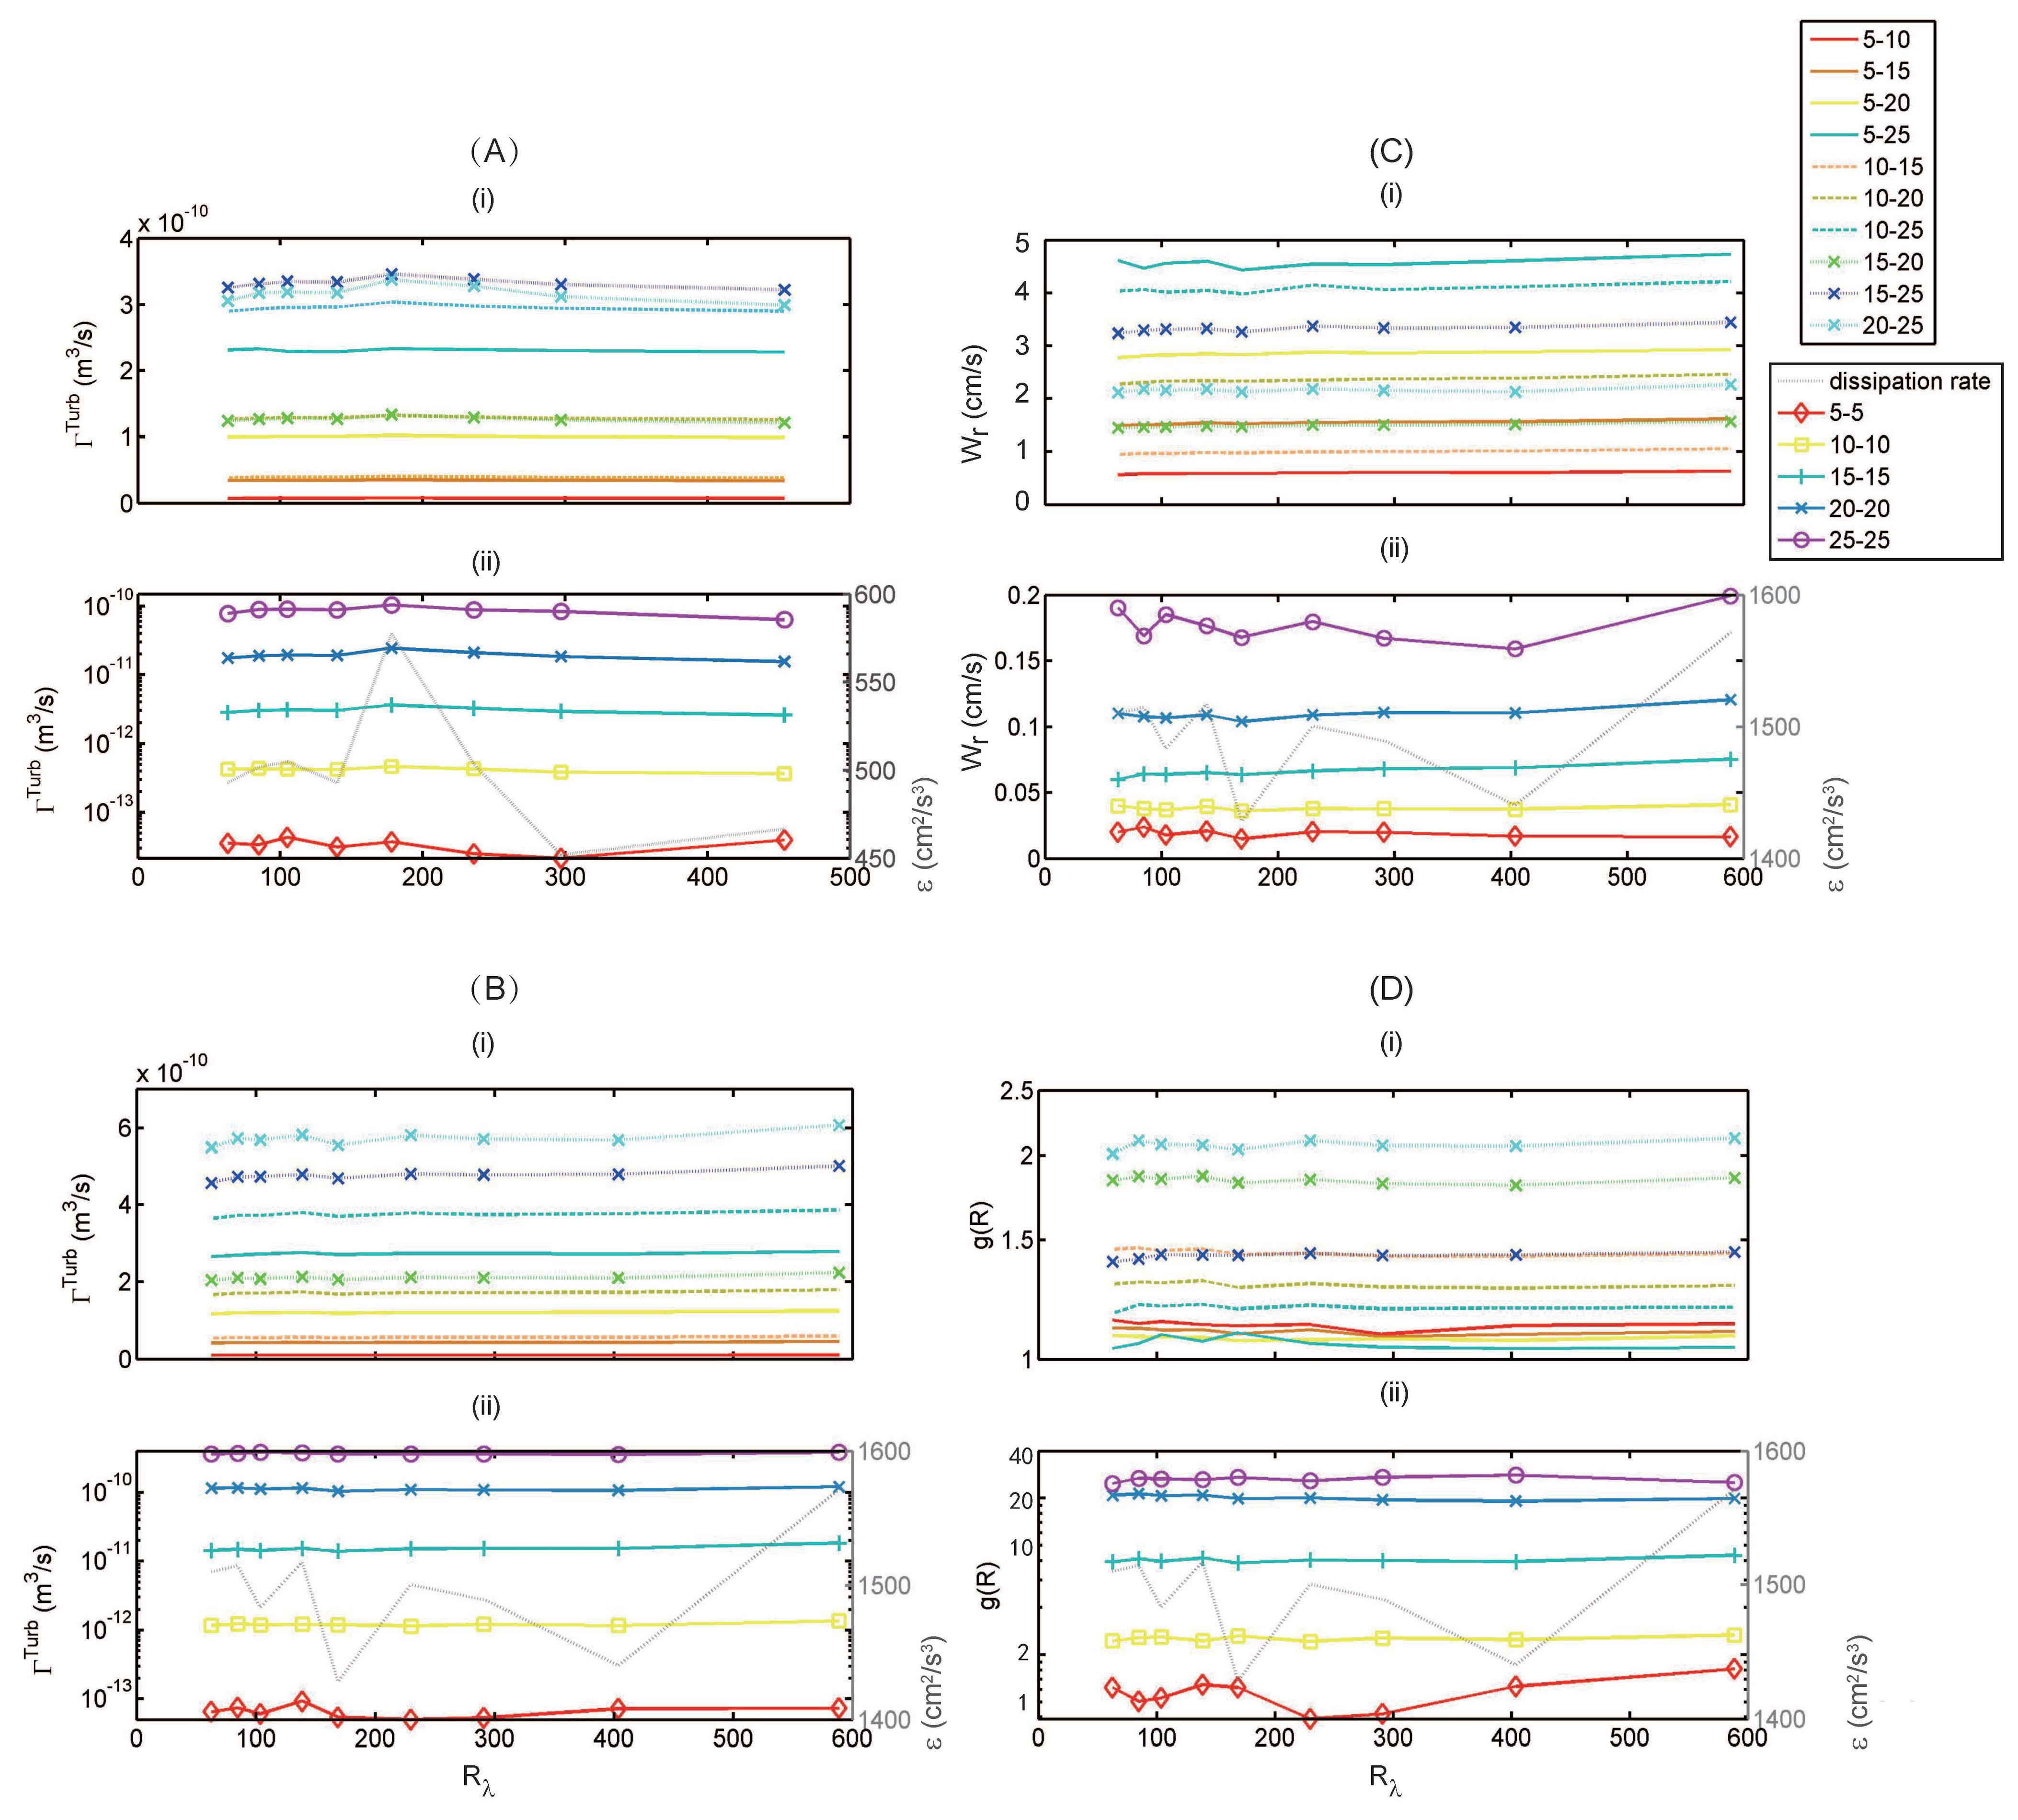
\includegraphics[width=\textwidth]{Figures/Chap2/re_cs.jpg}
\caption{ Collision statistics under different  $R_\lambda$ for all droplet pairs in this study. (A) and (B) are for collision kernels with $\epsilon \approx500$ cm$^2$ s$^{-3}$ and $\epsilon \approx1500$ cm$^2$ s$^{-3}$, respectively.  (C) and (D) are the same as (B) but for RRV and RDF, respectively. Results for cross-sized collisions are shown in (i)s and same-sized collisions in (ii)s. The gray dashed line depicts the EDRs under different simulations.} \label{fig:re_cs}
\end{figure}

\subsection{Collision statistics under different eddy dissipation rates} \label{sec:ch2_diss}

Since we have demonstrated that collision statistics are not sensitive to $R_\lambda$, we averaged over all resolutions in our studies to examine the effects of EDR. We found that all collision and pair statistics increase monotonically with EDR, which was consistent with the finding of \citet{Ayala2008a}. Among the three, RDF seemed to head towards an asymptotic value (figure \ref{fig:diss_cs} (b)).  The fluctuation of statistics among different resolutions grew slightly with increasing EDR, which can be attributed to the increasing intermittency of turbulence \citep[e.g. ][]{Pope2000}. 

\begin{figure}[ht]
\centering
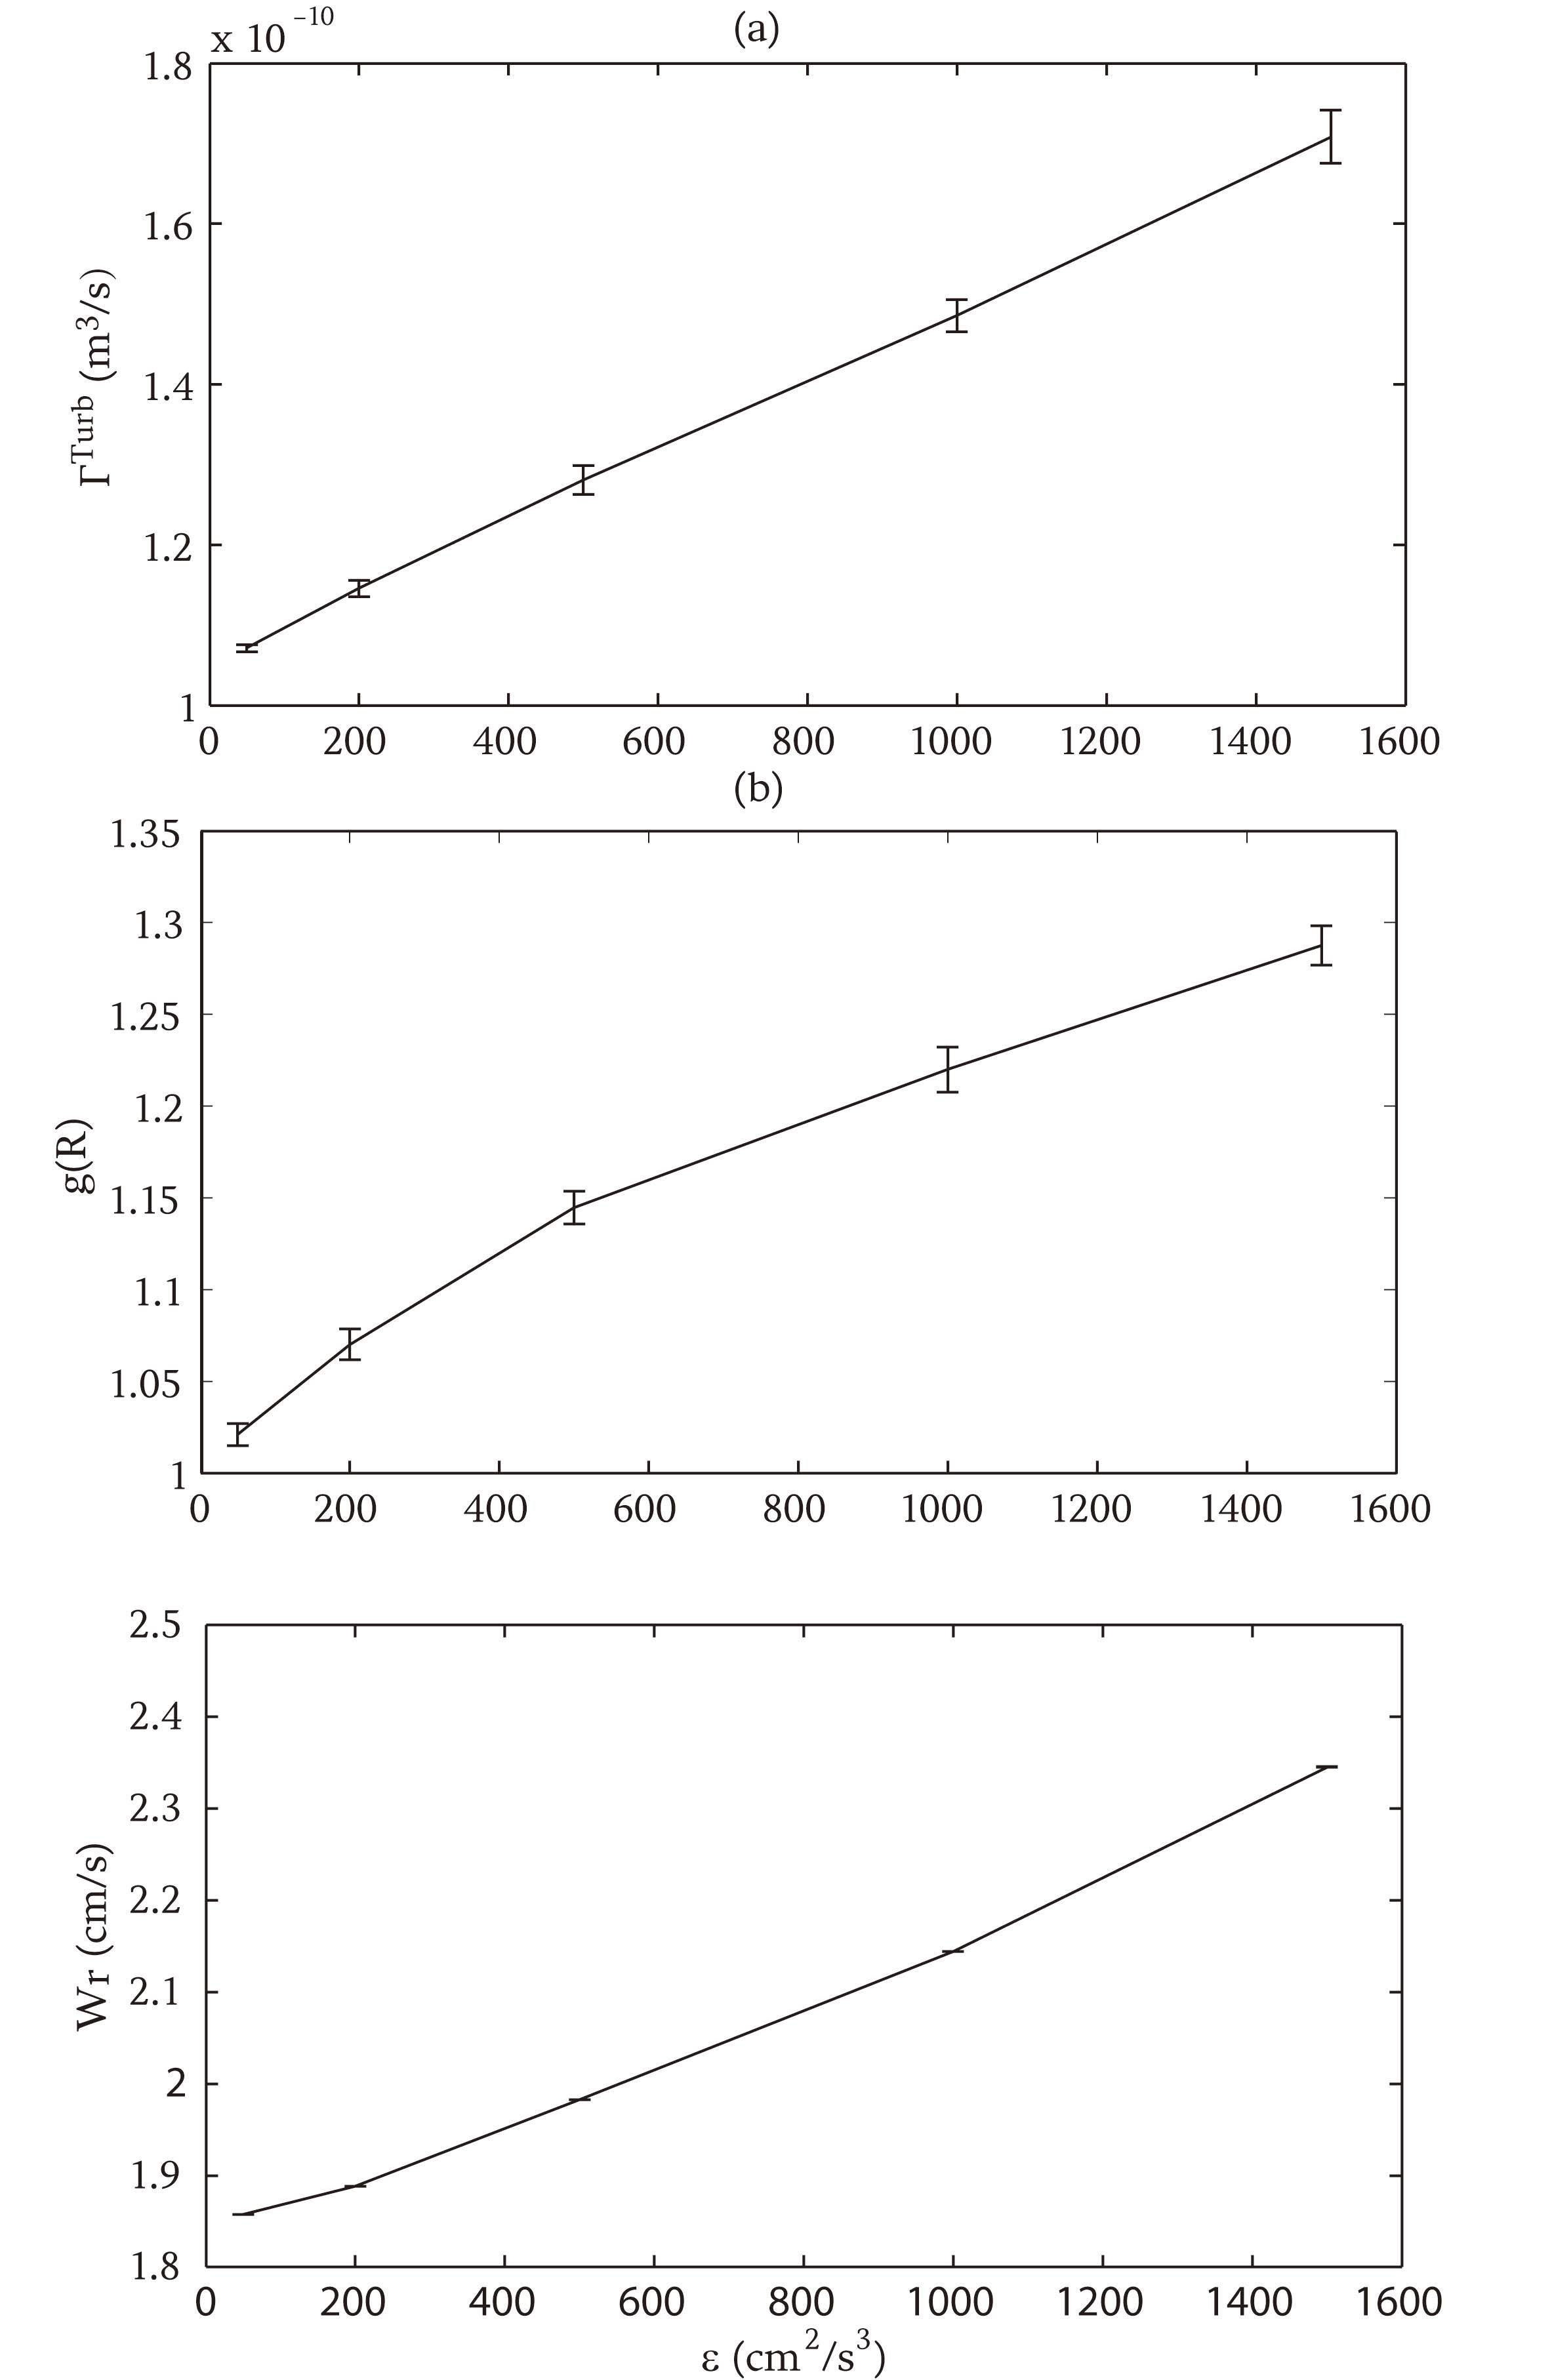
\includegraphics[width=0.8\textwidth]{Figures/Chap2/diss_cs.jpg} 
\caption{ Statistics of (a) collision Kernel, (b) RDF, and (c) RRV for droplets between 10 $\mu$m and 20 $\mu$m as a function of EDRs. The error bars show the standard deviation of the statistics with different $R_\lambda$-values} \label{fig:diss_cs}
\end{figure}

To better evaluate how EDR impacts the different droplet pairs, we normalized the statistics by their respective values in a purely gravitational setting. Since the results are insensitive to $R_\lambda$, or L, only simulations at one resolution  $N=256^3$ were examined. Figure \ref{fig:diss_cs_20_self} (a)-(c) showed that the cross-sized collision statistics involving 20 $\mu m$ droplets increased with EDR. The strongest enhancement in collision kernel occurs in the case of 20-25 $\mu$m droplet pairs, with a maximum enhancement of about 3.1 at the highest EDR. This increase was primarily attributed to the stronger clustering at high EDR, especially for the 20-25 $\mu$m droplet-pairs. Droplet pairs with similar size tended to cluster in the same regions of the flow due to similar droplet inertias and terminal velocities. This has been confirmed by previous studies \citep[e.g.,][]{Ayala2008a,Franklin2005}. An exception to this though, was pairs involving droplets with a radius $r = 5$ $\mu m$, that always seem to have a small value of RDF (see figure \ref{fig:diss_cs_20_self} (b)). This was probably due to the fact that small droplets have small Stokes numbers, indicating that they adjust very quickly to changes in the flow and therefore act more like fluid tracers than inertial droplets. The normalized RRV grew nearly linearly for all sizes with the strongest enhancement for 20-25 $\mu m$ pairs as well (figure \ref{fig:diss_cs_20_self} (c)). The results involving droplets of other sizes were similar and are thus not shown.

Same-sized collisions are impossible when gravity is the only influence on droplet motion because they have identical terminal velocities. However, when turbulence is present, collisions do occur. Before discussing the results it should be noted that there was a variation of about $3\%$ due to inadequate sampling, especially for droplets of $r=5$ $\mu m$ and 25 $\mu m$. The 5 $\mu m$ droplets had less chance to collide with one another due to their minute size and the 25 $\mu m$ droplets had the lowest concentrations among all the droplets, also leading to low collision rates. We can see from all panels of figure \ref{fig:diss_cs_20_self} that all three statistics increased with the size of droplet pairs, both for same-sized collisions and cross-sized collisions.

\begin{figure}[ht]
\centering
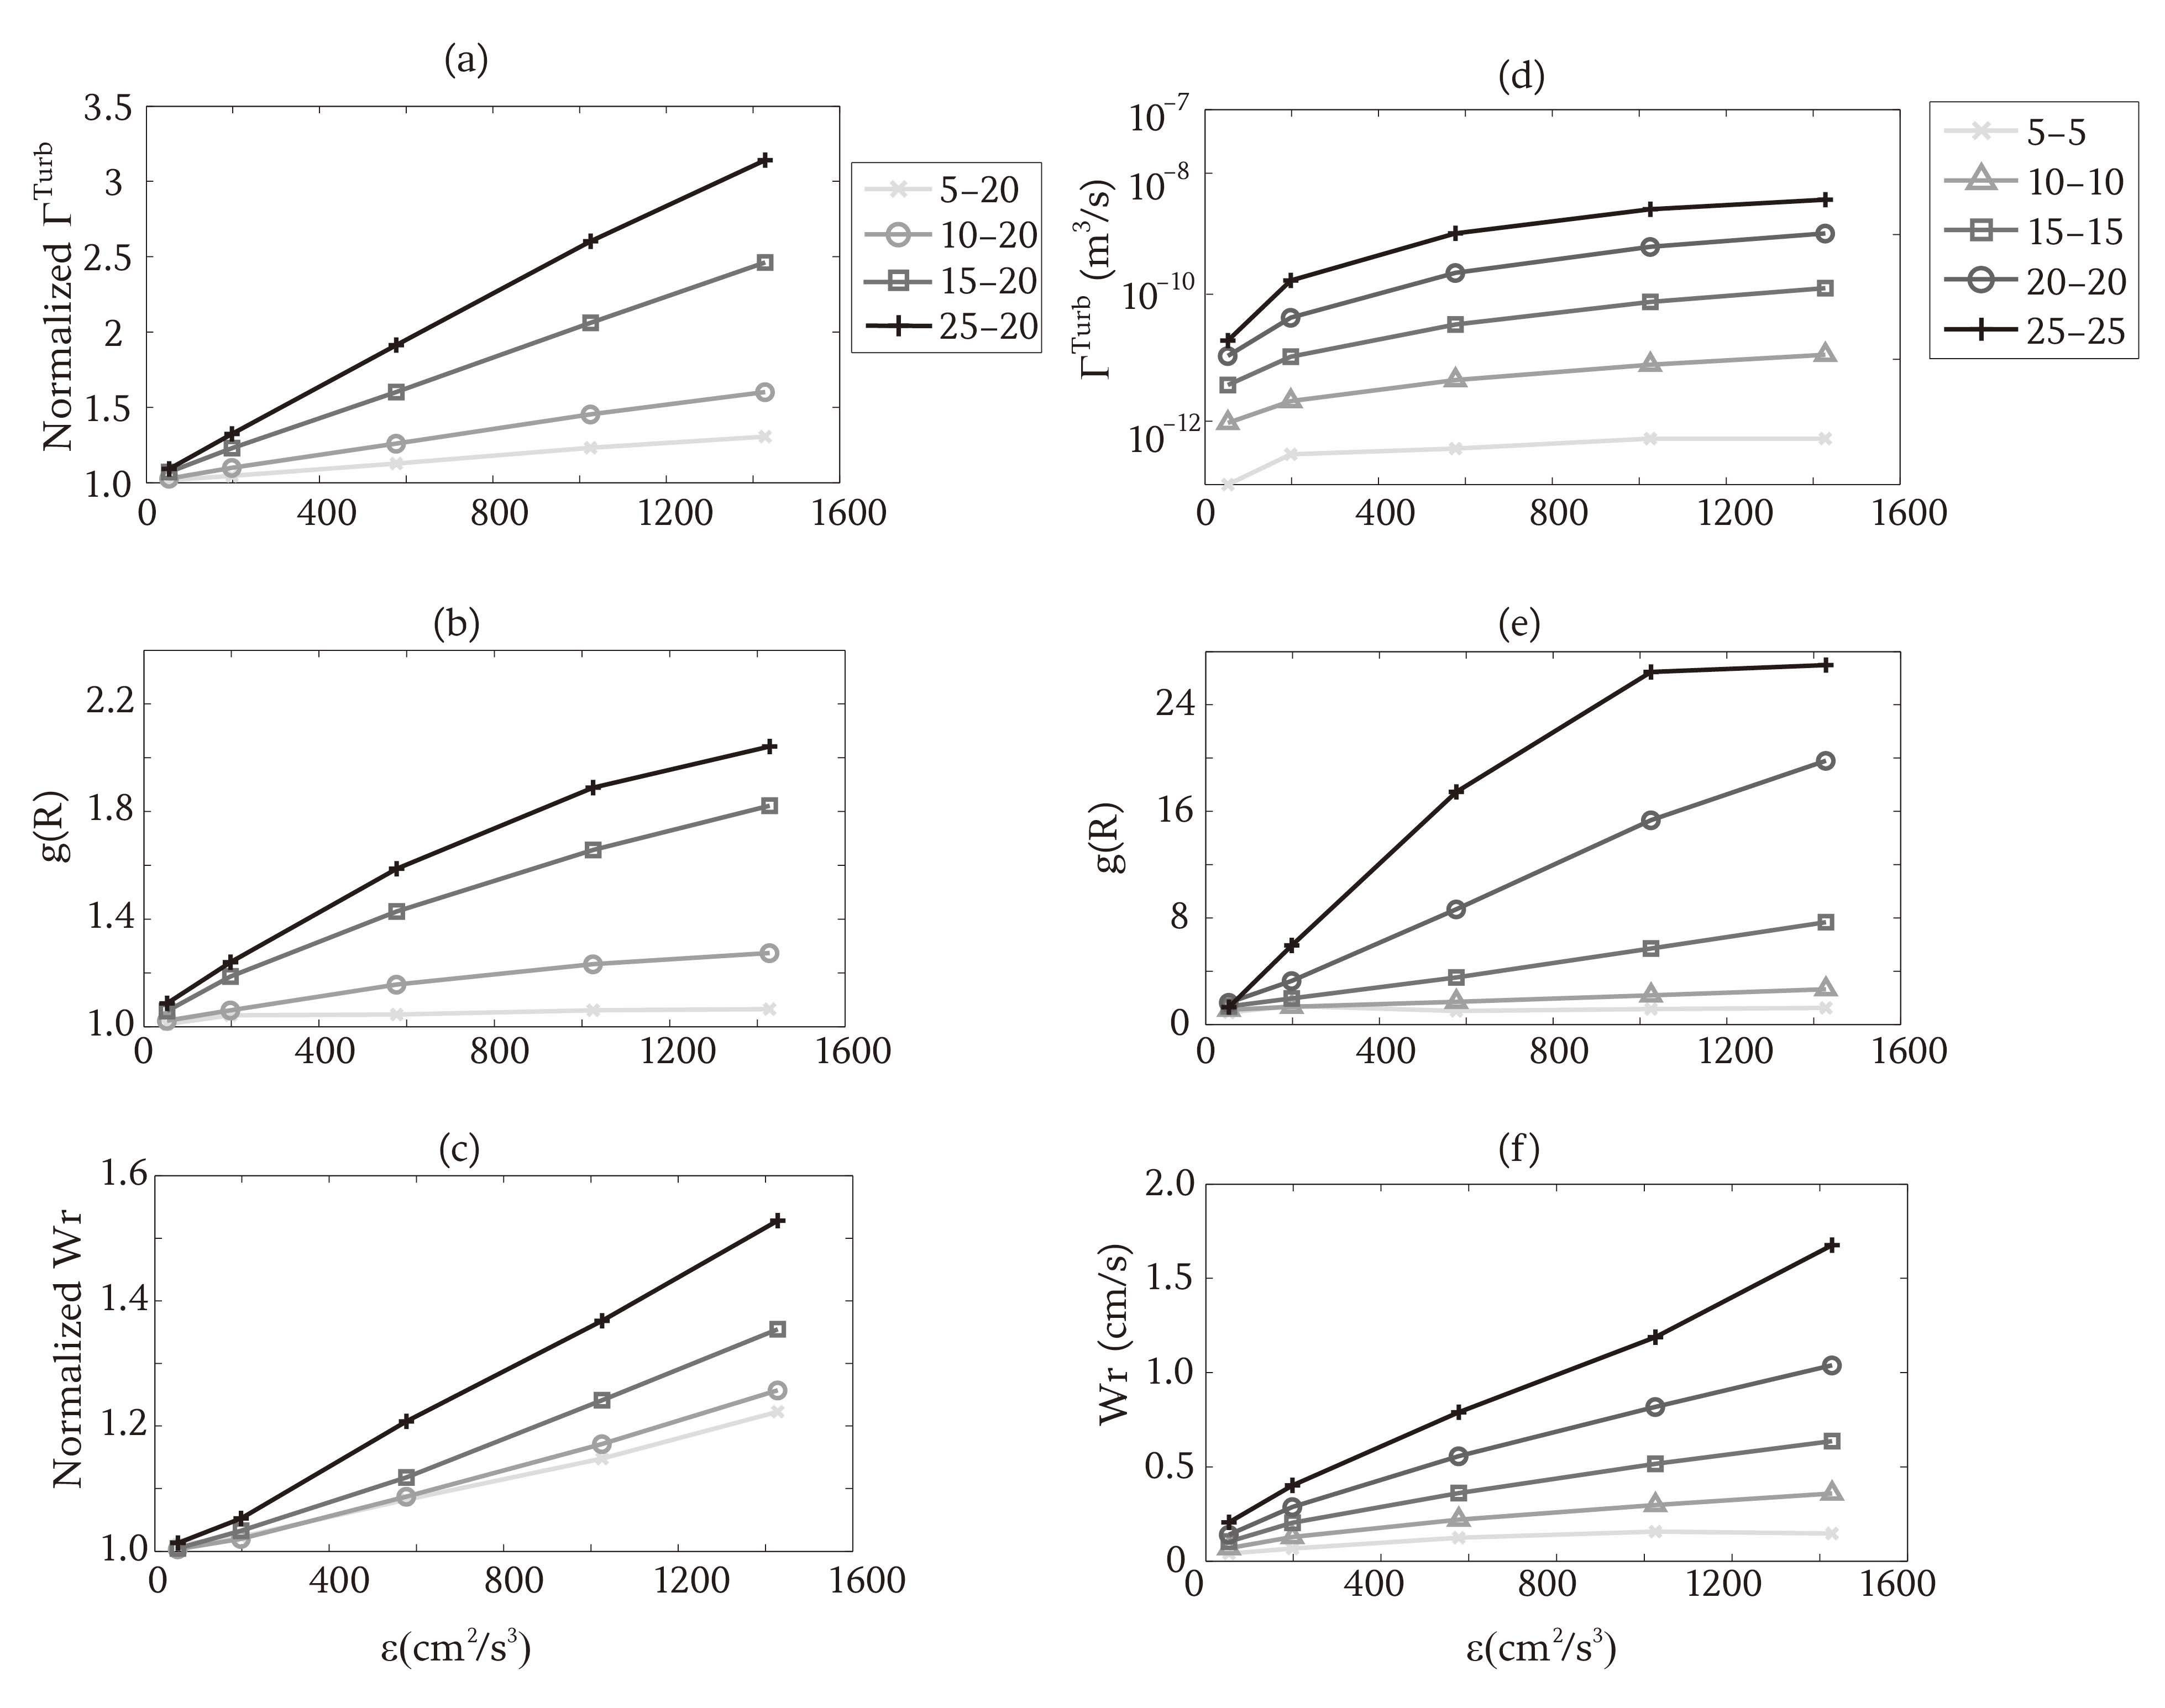
\includegraphics[width=0.8\textwidth]{Figures/Chap2/diss_cs_20_self.jpg} \caption{Collision statistics as a function of EDRs for cross-sized collisions involving 20 $\mu m$ droplets ((a)-(c)) and for same-sized collisions ((d)-(f)) } \label{fig:diss_cs_20_self}
\end{figure}

\section{Can we formulate a better collision parameterization?} \label{sec:ch2_parameterization}

We arrived at the conclusion that collision statistics for droplets of radius smaller than 25 $\mu m$ are insensitive to $R_\lambda$, implying the EDR and the pair sizes are the determining factors. As a consequence, we are of the opinion that parameterizations scaling with $R_\lambda$ are misleading. Here we introduce a modified parameterization scheme for turbulent collision kernels based on DNS data and at the same time attempt to match the forms of theoretical expressions from \citet{Saffman1956} and \citet{Wang1998b}.

\subsection{Turbulent collision kernel}

Given the dependence of the collision kernel on the EDR and droplet size, and the sensitivity test of $R_\lambda$ in section \ref{sec:ch2_result}, we applied curve fitting to our data to obtain a formula for the geometric collision kernel in the following form:
\begin{multline}
\Gamma^{Turb}=\Gamma^{Grav}+ 2\pi R^2 \Big[ \big(\frac{R}{\eta}\big)^{0.84}+(7 St_1 St_2)^{0.85}\Big]
 \times \sqrt{0.5\epsilon(|\tau_{p1}-\tau_{p2}|+0.3\sqrt{\tau_{p1}\tau_{p2}})}, \label{eqn:paragamma}
\end{multline}
where $St_i$ and $\tau_{pi}$ are the Stokes number and response time of the colliding droplets, respectively. The first term on the right-hand side is the gravitational collision kernel, which is $\pi R^2|V_{t2}-V_{t1}|$. The second term is the turbulence-enhanced component, which is the coupling of the clustering effect and the turbulent transport effect. The collision kernel, as demonstrated by DNS, is a function only of dissipation rate (as $\eta$ and $\tau_k$ can be derived from it) and droplet size; $R_\lambda$ and $u\prime$ are therefore excluded from the formula since they are both determined by the arbitrary size of the computational domain.

The predicted collision kernel calculated from the formula are shown in figure \ref{fig:parameterizations} (a) along with the results of our DNS. The parameterization reproduced the collision kernel correctly except for the case of same-sized collisions between 5 $\mu m$ droplets (the points in the lower left corner of the figure). Those collision events are not the major concern of our parameterization since they contribute very little to the overall droplet growth because of their low chance of colliding compared to other droplet pairs. Otherwise high accuracy in predicting the collision kernel is achieved by our parameterization. The relative error, which is calculated by normalizing the absolute difference between values from the parameterization and the DNS and taking the average, was used to measure the uncertainty of our parameterization scheme. The uncertainties came from a variety of sources. One was from poor sampling of same-sized collisions, especially for both the largest and smallest droplets, as mentioned in section \ref{sec:ch2_diss}; another source of uncertainty is simply the scatter resulting from finite-size ensembles of realizations.  The result shows that the uncertainty in predicting the cross-sized collision case was very small with a value of 6\%; however, for same-sized collisions, it was still significant (28\%). 


\subsection{Radial relative velocity}
\citet{Wang1998b} modified the analytical equation of RRV based on the studies of \citet{Saffman1956} and \citet{Hu1997} and proposed a more accurate formula:
\begin{multline}
\langle|\mathbf{W_r}|\rangle=\Big( \frac{2}{\pi} \Big)^{1/2}\bigg[ \frac{1}{15}R^2\frac{\epsilon}{\nu} + (\tau_{p2}-\tau_{p2})^2 \bigg\langle\bigg( \frac{Du}{Dt} \bigg)^2 \bigg\rangle \\
+ 2\tau_{p1}\tau_{p2} \bigg\langle \bigg( \frac{Du}{Dt} \bigg)^2 \bigg\rangle \frac{R^2}{\lambda_D^2} +\frac{\pi}{8}(\tau_{p2}-\tau_{p1})^2g^2\bigg]^{1/2}, \label{eqn:Wangpararrv}
\end{multline}
where $\frac{Du}{Dt}$ is the local fluid acceleration. $\lambda_D$ is the longitudinal Taylor microscale of fluid acceleration defined by $(\frac{1}{\lambda^2_D}) = -(1/2)\frac{\partial^2}{\partial x^2}f_D(0)$ and $f_D$ is the longitudinal correlation function of the velocity derivative. We fit curves to match our DNS data on the basis of their formula by keeping the local fluid shear term and gravity term (first and last term inside the square brackets) and modifying the fluid acceleration term and coupling term (second term and third term inside the square brackets) in a way that does not depend on $R_\lambda$ (i.e., without $\big\langle (\frac{Du}{Dt})^2\big\rangle$ and without the $\lambda_D$ term). The local fluid acceleration $\langle(\frac{Du}{Dt})^2\rangle$  and longitudinal Taylor microscale $\lambda_D$ are replaced with expressions involving EDR, which are the only way to use $\epsilon$ with $(\tau_{p1} - \tau_{p2})$ and $\tau_{p1}\tau_{p2}$ while keeping the same dimensions. We obtained the fit as follows:
\begin{multline}
\langle|\mathbf{W_r}|\rangle = \Bigg(\frac{2}{\pi}\Bigg)^{1/2} \Bigg\{\frac{1}{15}R^2\frac{\epsilon}{\nu} +\epsilon|\tau_{p2}-\tau_{p1}|\\
+ 0.001\epsilon\sqrt{\tau_{p1}\tau_{p2}}\bigg[ \bigg( \frac{R}{\eta}\bigg)^{0.1}-0.5 \bigg]
+\frac{\pi}{8}(\tau_{p2}-\tau_{p1})^2g^2 \Bigg\}^{(1/2)}, \label{eqn:pararrv}
\end{multline}
the first term inside the curly brackets measures the effect of local shear from turbulence, which is also the only remaining term when one considers only non-inertial particles. The second term denotes the different inertial response of the droplet pair to the local fluid acceleration. The third term is the overall response of the droplet pair due to local fluid acceleration, which is critical for same-sized collisions; the last term is the gravity term.  Figure \ref{fig:parameterizations} (b) demonstrates that the predicted RRV using the parameterization asymptotes to the observed value. For cross-sized collisions the gravity term has the largest contribution to RRV due to different terminal velocities; when colliding, droplet sizes get closer until they are equal, the gravitational effect diminishes and the local acceleration term (the third term) dominates. 

Our parameterization scheme for RRV performed with high accuracy for both the cross-sized collision case and the same-sized collision case. For cross-sized collisions, the average root-mean-square error (RMSE) of the normalized RRV (i.e. the RRV normalized by the value in the corresponding stagnant air case) was 0.03, which is much lower than \citet{Franklin2007}'s value of 0.28. The relative error was within 13\% which is slightly higher than that in \citet{Ayala2008b} (5\%). For same-sized collisions the relative error was 15\%, which improves upon \citet{Ayala2008b}'s parameterization where the relative error was 48\% for $\epsilon = 400 cm^2s^{-3}$. For a closer comparison, our relative error for $\epsilon = 500 cm^2s^{-3}$ was 14.73\%. Table \ref{tab:err} gives the relative errors of the collision statistics from our parameterization.

\subsection{Radial distribution function}
To quantify the clustering effects in a turbulent cloud system we also parameterized the RDF. We attempted to simply apply the analytical formula of the collision kernel \eqref{eqn:sph}. Therefore, $g(R)= \frac{\Gamma^{Turb}}{(2\pi R^2 \langle |\mathbf{W_r}| \rangle )}$, where $\Gamma^{Turb}$ and $\langle |\mathbf{W_r}| \rangle$ were obtained from the parameterizations derived in the previous section. However, the quotient of $\Gamma^{Turb}$ and $\langle |\mathbf{W_r}| \rangle$ led to amplified error. Even though the average relative error was small (0.19), the parameterized RDF had a group of values below unity, which is unreasonable. Therefore this simple method was proved incapable to evaluate the clustering effects in a quantitative sense, but it can still help to make a qualitative assessment, which is easier to calculate than the following method we will introduce. 

\citet{Ayala2008b} developed an empirical formula for g(R) that includes both same-sized collisions and cross-sized collisions (see equation \eqref{eqn:parardf}  below). However their parameterization is a function of $R_\lambda$. This caused a spread of g(R) under the same EDR but over a broad range of $R_\lambda$. The average error using this method was 0.18 and was largely caused by the spread. To remove the $R_\lambda$ effect, we modified their formula by replacing the terms that contained $R_\lambda$ with constants in order to fit our data. The overall structure was the same but the calculation of terms of $r_c$ and $C_1$ was simplified. $r_c$ and $C_1$ depended on the $R_\lambda$ in their original paper. Here we used constants to replace those terms and their formulas are given below: 
\begin{equation}
g(R)=(\frac{\eta^2+r_c^2}{R^2+r_c^2})^{C_1/2}, 
 \label{eqn:parardf}
\end{equation}

\begin{equation}
C_1=\frac{y(St)}{[|{\bf g}|/(v_k/\tau_k)]^{0.36}},
\end{equation}

\begin{equation}
(\frac{r_c}{\eta})^2=|St_1-St_2|\times F,
\end{equation}

\begin{equation}
F=20.115 \times \Big[{\frac{15 + \frac{\pi}{8}\big(\frac{|\bf{g}|}{v_k/\tau_k}\big)^2}{200}}\Big]^{1/2}.
\end{equation}

Here $y(St)$ is a fitted polynomial function of $St$ fitted based on their DNS experiments; $v_k = (\nu\epsilon)^{1/4}$ is the Kolmogorov velocity. 

The parameterized $g(R)$ matched well the simulations with an average relative error of 0.12 (see figure \ref{fig:parameterizations}(c)). The red dots from the DNS simulations with values below 1 originated in 5-5 $\mu m$ collisions and were caused by poor sampling as these droplets have little possibility to collide with each other and their pair statistics were based on less than 3000 collisions. 

\begin{table}[ht]
\caption{Relative errors for the parameterization of the collision statistics, for same-sized collisions, cross-sized collisions, and the average for all collisions\strut} \label{tab:err}
\begin{center}
\def\arraystretch{1.5}
\begin{tabular}{cccc}
\hline\hline
 & Same-sized collision & Cross-sized collision & Average \\
\hline
$\Gamma^{Turb}$ & 0.28 & 0.06 & 0.14\\
\hline
$\mathbf{W_r} $ & 0.15 & 0.13 & 0.14 \\
\hline
g(R) & 0.21 & 0.07 & 0.12 \\
\hline
\end{tabular}
\end{center}
\end{table}
\begin{figure}[ht]
\centering
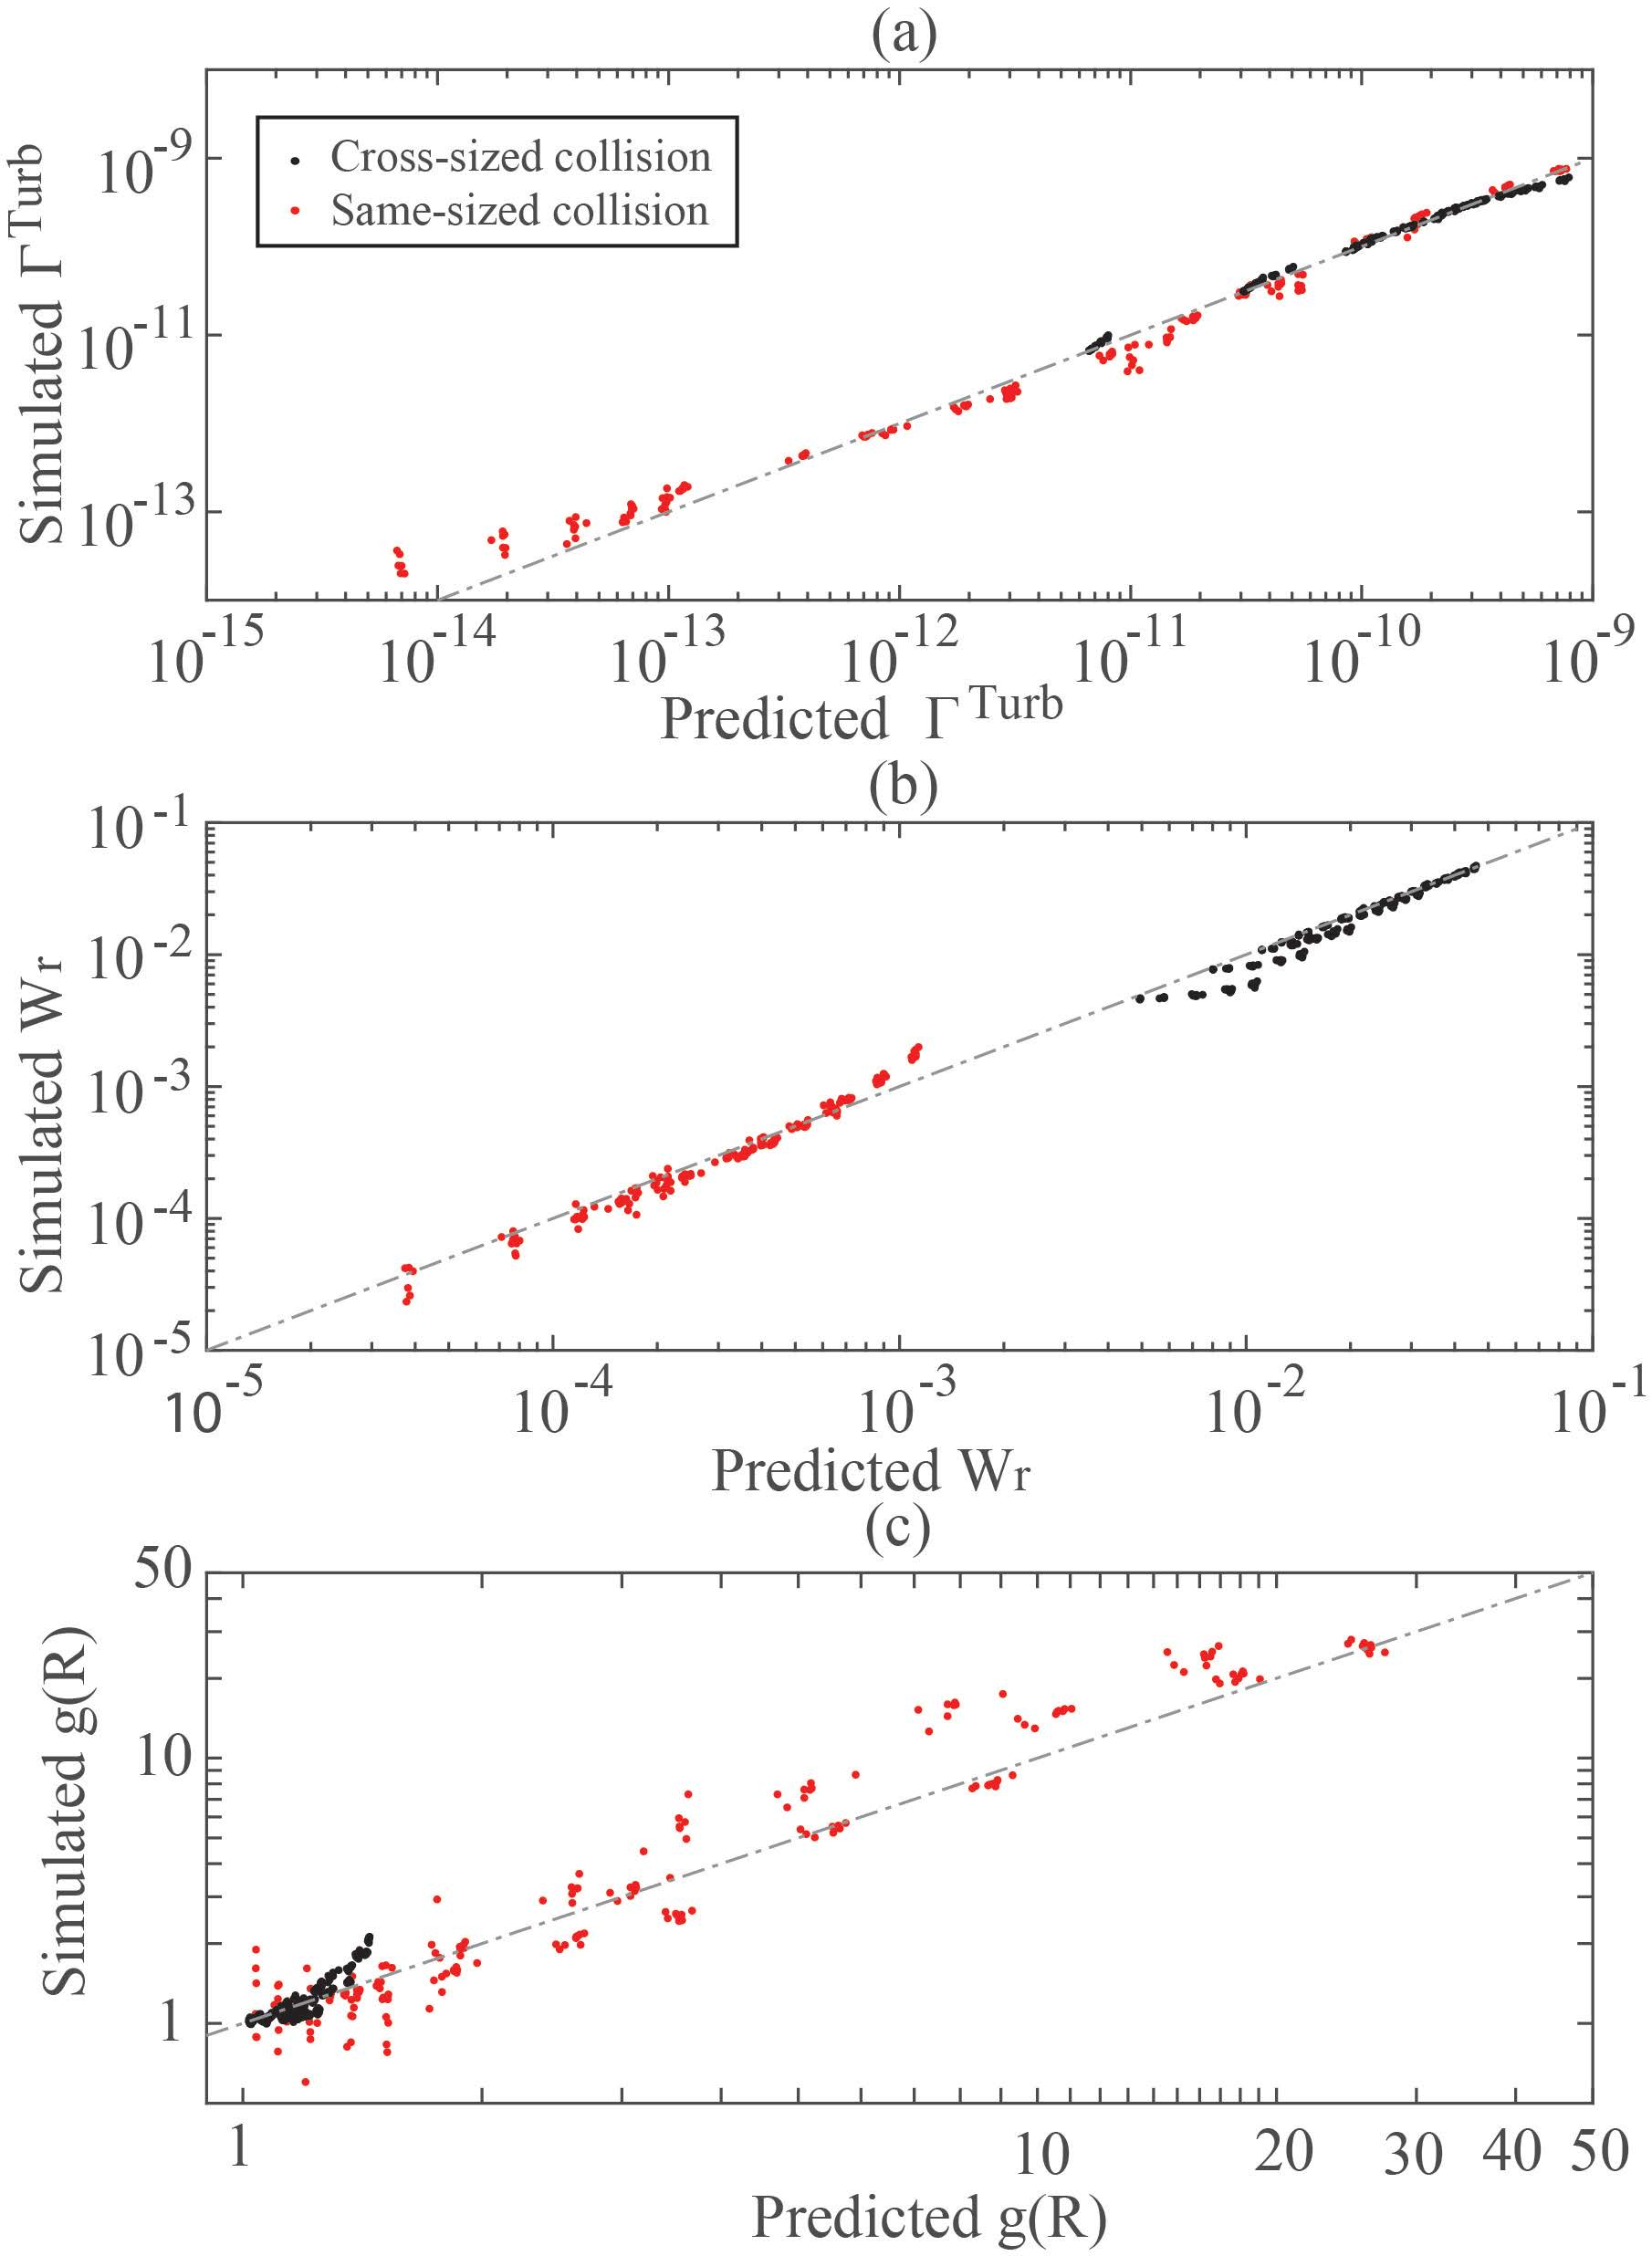
\includegraphics[width=0.6\textwidth]{Figures/Chap2/parameterizations.jpg}\\
\caption{(a) collision kernel ($m^3 s^{-1}$), (b)  RRV ($cm s^{-1}$), and (c) RDF from the DNS against their corresponding parameterized value for cross-sized collisions (black dots) and same-sized collisions (red dots). Different dots represent statistics of different droplet pairs with different turbulent conditions.} \label{fig:parameterizations}
\end{figure}

\subsection{Comparisons with DNS data and other models}
In this section, a brief comparison of our prediction model with other studies \citep{Franklin2007, Saffman1956, Wang1998b, Zhou2001, Ayala2008b} is given. We compared the turbulence enhancement of the collision kernel between 10 $\mu m$ - 20 $\mu m$ droplets and that of 10 $\mu m$ - 15 $\mu m$ with different eddy dissipation rates. 

The DNS results of \citet{Ayala2008a} were obtained from their largest $R_\lambda$(=72.4) case where we assumed sufficient scale separation has been achieved such that $R_\lambda$ does not affect the collision statistics. Figure \ref{fig:colker} shows that the difference between our DNS results and their results was insignificant. The collision kernel from \citet{Franklin2005} grew faster than the other models by a factor of 1.65 due to the difference in calculating flow parameters, discussed in section \ref{sec:ch2_flowpara}, suggesting that their parameterization yields significant overestimation of the collision kernel (see blue dashed line in figure \ref{fig:colker}). The studies from \citet{Wang1998b} and \citet{ Saffman1956} did not consider the clustering effect and consequently underestimate the values (see dashed curves with light green and gray, respectively). The RDF by \citet{Zhou2001} was parameterized based on a non-sedimenting assumption. Thus one would expect some overestimation \citep{Xue2008} because droplets would stay in clouds longer without sedimentation. However, even after including the clustering effect given by \citet{Zhou2001}, the curve of \citet{Wang1998b} was still lower than the DNS data, even though it displayed a similar slope (see dark green curve in figure \ref{fig:colker}). 
\citet{Pinsky2006collision} developed a model in which the turbulence was represented using a statistical formulation. Therefore, large Reynolds numbers were achieved in their study. Since their model did not include clustering effects, underestimation was expected in the collision kernel. We compared their curve of collision kernel of 10-15 $\mu m$ pair statistics with the DNS data (not shown in figure); larger underestimation was found at low intensities (stratiform clouds and cumulus clouds as categorized by their paper in the bottom of figure 7). By contrast, our parameterization scheme performed well at low EDRs and deviated slightly from the DNS data as the dissipation rate became higher (see figure \ref{fig:colker}), implying a good performance in predicting stratiform to cumulus clouds (with an EDR less than $\approx 600 cm^2s^{-3}$).  Overall, most of the parameterization schemes underestimated the turbulent enhancement except for the curve of \citet{Ayala2008b} (purple dashed curve). Although our parameterization showed some uncertainties, its results still show a good fit to the DNS.

\begin{figure}[ht]
\centering
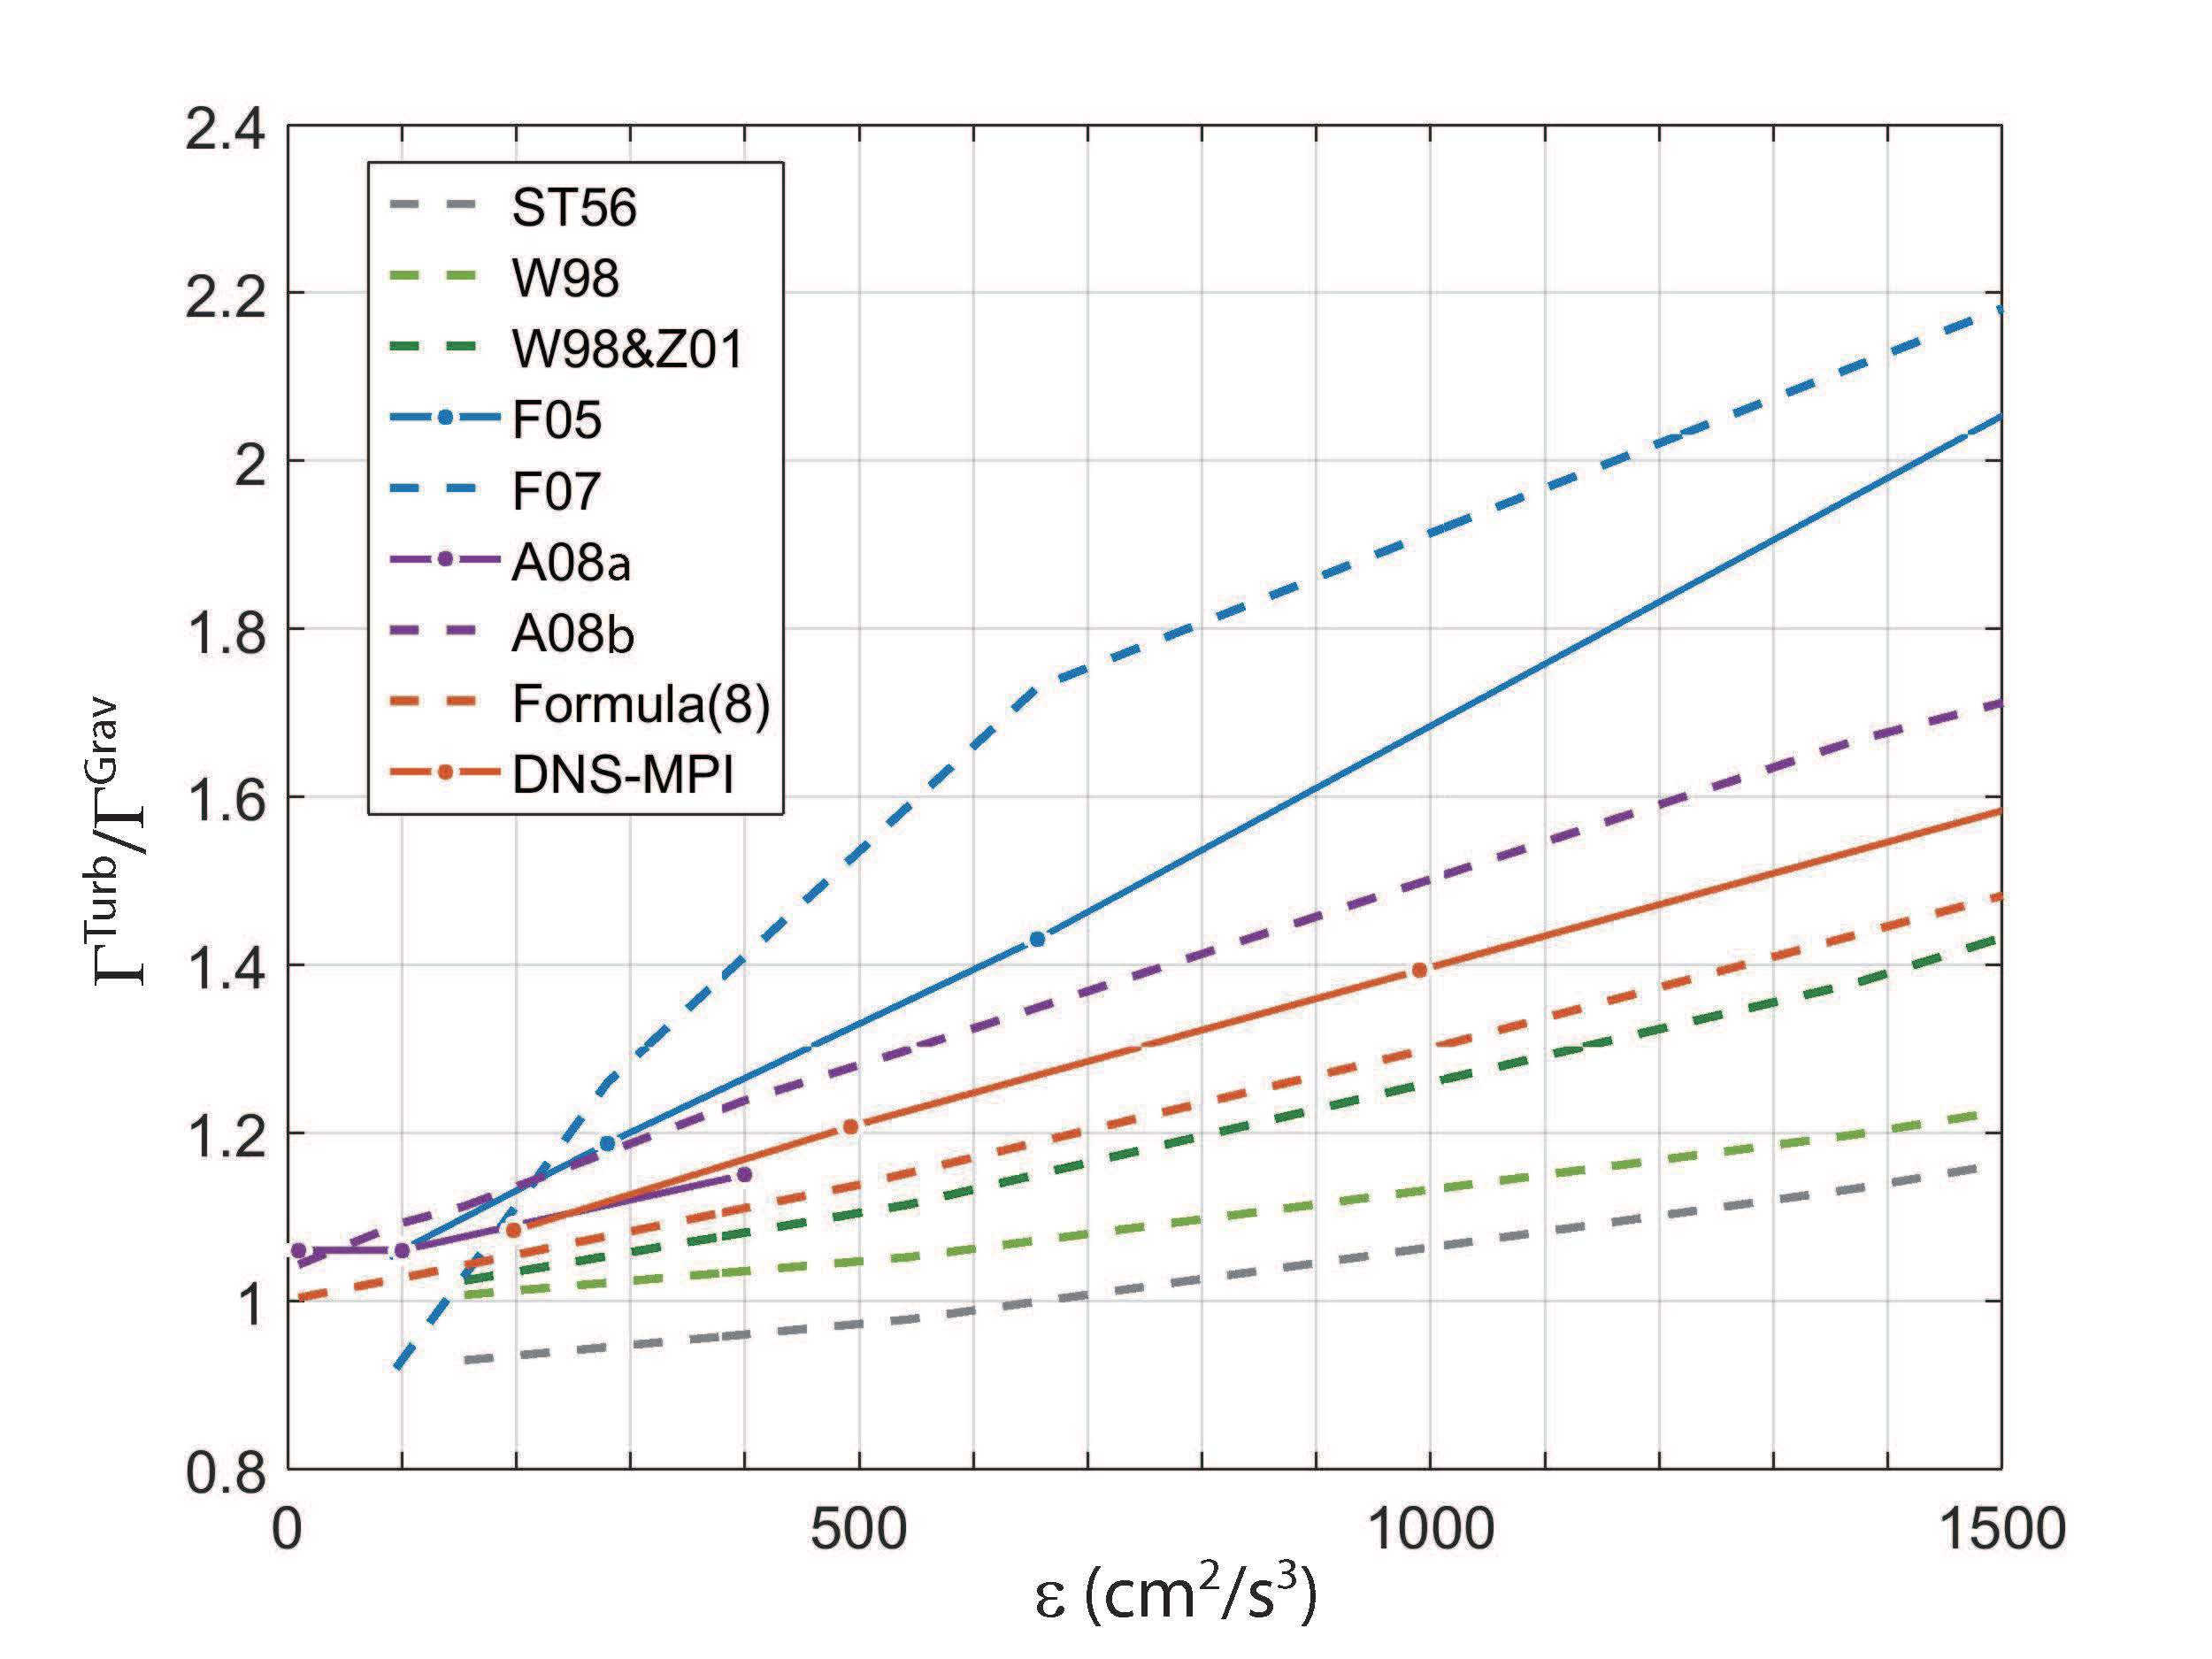
\includegraphics[width=0.7\textwidth]{Figures/Chap2/compares.jpg}  \\
\caption{Ratio of turbulent collision kernel and gravitational collision kernel for droplet pairs of 10-20 $\mu m$ as a function of EDRs from different studies \citep{Saffman1956, Wang1998b, Zhou2001, Ayala2008a, Ayala2008b, Franklin2005, Franklin2007}. Solid lines represent results obtained from simulations of various models; dashed lines represent parameterized values; different colors marks different studies. The lines in brown are from this study. }\label{fig:colker}
\end{figure}

\section{Summary and discussion} \label{sec:ch2_conclusion}

In this study we examined the major question of warm rain initiation: what role does turbulence play in droplet collisional growth? And can we obtain a more accurate parameterization? With the help of DNS, we quantified the turbulence effect in droplet growth by collision-coalescence based on 39 successful runs (including five different eddy dissipation rates and nine different Reynolds numbers or computational box sizes) with 15 different combinations of droplet pairs in the appropriate range for real clouds to initiate collision-coalescence processes. We studied three collision statistics (RRV, RDF, and turbulent collision kernel) between droplets of radius less than 25 $\mu m$ using a model configuration different from \citet{Franklin2005}, which allowed us to successfully separate the effect of $R_\lambda$ from $\epsilon$, or EDR. We found that all collision statistics were insensitive to $R_\lambda$ over the range of box sizes we can afford to simulate and as long as the model resolved all the smallest scales of turbulence (i.e., the Kolmogorov length scale). This implies that the droplet motions and their collision statistics are mainly affected by the smallest fluid scales, and that the large-scale motion has negligible influence. Moreover, the collision statistics were found to be strongly correlated with the EDR and the size of droplets. Therefore, we developed a parameterization, which is independent of $R_\lambda$ and $u\prime$ and instead is dependent on turbulence intensity ($\epsilon$ or EDR), the fluid properties ($\rho_a, \nu$, etc.), and the droplet sizes. 

We proposed a form of the collision kernel that includes both same-sized collisions and cross-sized collisions and thus is able to describe the continous growth of droplets by collisions. The parameterized collision kernel was demonstrated to be highly consistent with DNS results. The formula predicted the turbulent collision kernel with an error of 15\% on average, better than other proposed formulas. We also parameterized the RRV and RDF, which offers future model developers a measure of the turbulence effect on the relative motion and spatial distribution of droplets. Their average relative errors were 14\% and 16\%, respectively. Again, an improvement over previous studies. 

It is recognized that the droplet growth rate is also determined by other factors such as the collision efficiency and condensational growth. To accurately parameterize the effect of turbulence on cloud droplet growth, the next step is to include these mechanisms. 

\acknowledgments
Computations were mainly made on the supercomputer Mammouth II parall\`{e}le from Universit\'{e} de Sherbrooke, managed by Calcul Qu\'{e}bec and Compute Canada. The operation of this supercomputer is funded by the Canada Foundation for Innovation (CFI), NanoQu\'{e}bec, RMGA and the Fonds de recherche du Qu\'{e}bec - Nature et technologies (FRQ-NT). Part of the simulations were run on the supercomputer SGI Altix 4700 from Universit\'{e} de Montr\'{e}al. This work was supported by the Natural Sciences and Engineering Research Council of Canada (NSERC). 

\cleardoublepage 
